%\documentclass{revtex4-1}
% options: aip, jcp, reprint, preprint
\documentclass[preprint]{revtex4-1}
%\documentclass[aip,jcp,reprint,superscriptaddress]{revtex4-1}

\usepackage{amsmath}
\usepackage{amsthm}
\usepackage{mathrsfs}
\usepackage{graphicx}
\usepackage{dcolumn}
\usepackage{bm}
\usepackage{multirow}
\usepackage{hyperref}
\usepackage{tikz}
%\usepackage{setspace}

\tikzstyle{blackdot}=[circle,draw=black,fill=black,
                      inner sep=0pt,minimum size=1.5mm]
\tikzstyle{whitedot}=[circle,draw=black,fill=white,
                      inner sep=0pt,minimum size=1.5mm]
\tikzstyle{combine}=[green!30!black, very thick, densely dotted]
\tikzstyle{concat}=[blue!40!black, very thick, densely dashed]

\numberwithin{equation}{subsection}
\renewcommand{\theequation}{\thesection.\thesubsection.\arabic{equation}}

\numberwithin{table}{section}
\renewcommand{\thetable}{\thesection.\arabic{table}}

\newtheorem{defn}{Definition}
\newtheorem{thrm}{Theorem}
\newtheorem{lemm}[thrm]{Lemma}
\newtheorem{prop}[thrm]{Proposition}

\newcommand{\vct}[1]{\mathbf{#1}}
\providecommand{\vr}{} % clear \vr
\renewcommand{\vr}{\vct{r}}
\newcommand{\vk}{\vct{k}}
\newcommand{\vR}{\vct{R}}
\newcommand{\dvr}{d\vr}
\newcommand{\dvR}{d\vR}
\newcommand{\dvk}{\frac{d\vk}{(2\pi)^D}}
\newcommand{\tdvk}{\tfrac{d\vk}{(2\pi)^D}}

% add a superscript ``ex''
\newcommand{\supex}[1]{ { { #1 }^{ \mathrm{ex} } } }
\newcommand{\Pex}{\supex{P}}
\newcommand{\Fex}{\supex{F}}
\newcommand{\muex}{\supex{\mu}}
\newcommand{\kex}{\supex{\kappa}}
\newcommand{\Chn}{\mathscr{C}}
%\newcommand{\Chn}{\mathcal{C}}
%\newcommand{\Chn}{\mathsf{C}}
\newcommand{\secref}[1]{Sec. \ref{#1}}

\newcommand{\FT}{\mathscr{F}}

\newcommand{\llbra}{[\![}
\newcommand{\llket}{]\!]}





\begin{document}

\title{Notes on ``computation of virial coefficients from integral equations''}
\author{Cheng Zhang, Chun-liang Lai, B. Montgomery Pettitt}

\maketitle

\tableofcontents




\section{Main text: Methods}


\subsection{Fourier-space OZ relation, from Eq. (2) to (3)}

In the real space, the Ornstein-Zernike (OZ) relation
is expressed as a convolution:
\begin{align}
  t(\vr)
&= \rho \, (c*h)(\vr)
= \rho \, \int c(\vr') \, h(\vr - \vr') \, d\vr'
  \tag{2}
  \label{eq:oz}
\end{align}
The convolution in the Fourier space is a product:
\begin{align}
  \tilde{t}(\vk)
&= \int_\vr t(\vr) \, e^{-i\vk \cdot \vr} \, d\vr
  \notag \\
&= \rho \int_\vr \int_{\vr'} c(\vr') h(\vr - \vr') d\vr' e^{-i\vk \cdot \vr} \, d\vr
  \notag \\
&= \rho \int_\vr' c(\vr') e^{-i\vk \cdot \vr'} \, d\vr'
        \int_\vR h(\vR) e^{-i\vk \cdot \vR} \, d\vR
  \notag \\
&= \rho \, \tilde{c}(\vk) \, \tilde{h}(\vk).
  \tag{3}
  \label{eq:ozk}
\end{align}
%
Here $\vR \equiv \vr - \vr'$.



\subsection{OZ relation, from Eq. (3) to Eq. (10)}

The density component form of \eqref{eq:ozk} satisfies
\begin{align*}
  \sum_{l = 1}^{\infty} \tilde{t}_l \, \rho^l
  &=
  \rho \sum_{i = 0}^{\infty} \tilde{c}_i \rho^i
  \sum_{j = 0}^{\infty} \tilde{h}_j \rho^j
  \quad \mbox{set ($i \rightarrow l - 1 - j$)}
  \\
  &=
  \sum_{l = 1}^{\infty}
  \left(
  \sum_{j = 0}^{l-1}
    \tilde{c}_{l-1-j} \tilde{h}_j \right) \rho^l.
\end{align*}

So
\begin{equation}
  \tilde{t}_l(\vk)
= \sum_{j = 0}^{l - 1}
  \tilde{c}_{l-1-j}(\vk) \, \tilde{h}_j(\vk).
  \tag{10}
\end{equation}



\subsection{$c(\vr)$ from the closure, from Eq. (4) to Eq. (11)}

From
\begin{equation}
  c(\vr) = [f(\vr) + 1] \, y(\vr) - 1 - t(\vr),
  \tag{4}
  \label{eq:closure}
\end{equation}
we have
\[
  \sum_{l = 0}^{\infty} c_l \rho^l
= (f + 1) \sum_{l = 0}^{\infty} y_l \rho^l
  - 1 - \sum_{l = 1}^{\infty} t_l \rho^l,
\]
which shows
\begin{equation}
  c_l(\vr) = [f(\vr) + 1] \, y_l(\vr) - t_l(\vr) - \delta_{l, 0},
  \tag{11}
  \label{eq:closurel}
\end{equation}



\subsection{PY closure, from Eq. (6) to Eq. (12)}



The PY closure is
\begin{equation}
  y(\vr) = 1 + t(\vr).
  \tag{6}
  \label{eq:pyclosure}
\end{equation}
So
\[
  \sum_{l = 0}^{\infty} y_l \rho^l = 1 + \sum_{l = 1}^{\infty} t_l \rho^l,
\]
which shows $y_l = t_l + \delta_{l, 0}$.
%
Using this in \eqref{eq:closurel} yields
\begin{equation}
  c_l(\vr) = f(\vr) \, [t_l(\vr) + \delta_{l, 0}].
  \tag{12}
\end{equation}



\subsection{Compressibility-route $B_n^{(c)}$, from Eq. (13) to Eq. (14)}



The compressibility equation of state is
\begin{equation}
  \partial_\rho (\beta \, P) = 1 - \rho \int c(\vr) \, d\vr.
  \tag{13}
  \label{eq:compr}
\end{equation}

Compressibility-route virial coefficient
\[
  \partial_\rho \left( \sum_{n = 1}^\infty B_n \rho^n \right)
=
  1 - \rho \int \left( \sum_{l = 0}^\infty c_l(\vr) \rho^l \right) \, d\vr,
\]
%
which means
%
\[
  \sum_{n = 1}^\infty n B_n \rho^{n - 1}
=
1 - \sum_{l = 0}^\infty \left( \int c_l(\vr) \, d\vr \right) \rho^{l+1}.
\]
Setting $l = n - 2$ yields
\begin{equation}
  B_n = -\frac{1}{n} \int c_{n-2}(\vr) \, d\vr.
  \tag{14}
  \label{eq:Bncompr}
\end{equation}



\subsection{Eq. (15)}

Taking the gradient of
\[
  f(\vr) = e^{-\beta \phi(\vr)} - 1,
\]
yields
\[
  \nabla f(\vr) = -\beta \nabla \phi(\vr) \, e^{-\beta \phi(\vr)}.
\]
So
\[
  \nabla f(\vr) y(\vr) = -\beta \nabla \phi(\vr) g(\vr).
\]



\subsection{Virial-route $B_n^{(v)}$, Eq. (16)}



Virial-route virial coefficient
\[
  \nabla f =
  \left(
  \frac{ \partial f }
       { \partial x_1 },
  \dots,
  \frac{ \partial f }
       { \partial x_D }
  \right)
  =
  \left(
  \frac{ x_1 } { r },
  \dots,
  \frac{ x_D } { r }
  \right)
  \frac{ d f(r) }
       { d r },
\]
where we have used that $\partial r / \partial x_i = x_i / r$
(Differentiating $r^2 = \sum_{i = 1}^D x_i^2$
 yields $2 r dr = \sum_{i = 1}^D 2 x_i d x_i$,
 or $dr = \sum_{i = 1}^D (x_i/r) \, d x_i$).

So
\[
  \vr \cdot \nabla f
=
  \frac{
    \sum_{i = 1}^D x_i^2
  } { r }
  f'(r) = r f'(r).
\]

Now the density expansion of
\begin{equation}
  \beta \, P
= \rho
  + \frac{\rho^2 \, \beta } {2 D}
  \int (\vr \cdot \nabla f) \, y(\vr) \, d\vr
  \tag{15}
\end{equation}
is given by
\[
  \sum_{n = 1}^\infty B_n \rho^n
= \rho
+
\frac{ \rho^2 }{ 2 D }
\int r f'(r)
    \sum_{l = 0}^\infty y_l(\vr) \rho^l \, d\vr.
\]
%
Setting $n = l + 2$ yields
\begin{equation}
B_n = \frac{1}{2D} \int r f'(r) y_{n-2}(r) \, d\vr.
\tag{16}
\end{equation}



\subsection{Hard-sphere $B_n^{(v)}$, Eq. (17)}


Eq. (17) states that
\begin{equation}
  B_n^{(v)} = B_2 \, y_{n-2}(1).
  \tag{17}
  \label{eq:BnB2y}
\end{equation}
%
To show this, we start with
\begin{align}
  B_n^{(v)}
&=
  \frac{1}{2D}
    \int_0^\infty r f'(r) y_{n-2}(r) S_D(r) \, dr
    \notag \\
&=
  \frac{1}{2D}
    \int_0^\infty r \delta(r - 1) y_{n-2}(r) S_D(r) \, dr
    \notag \\
&= \frac{1}{2D}
    y_{n-2}(1) S_D(1),
    \label{eq:Bnv}
\end{align}
%
where $S_D(r)$ is the surface area,
which is equal to $4\pi r^2$ in three dimensions,
or Eq. \eqref{eq:surfareaD} in general.

Now applying the above formula to the $n = 2$ yields
\begin{equation}
B_2^{(v)}
=
\frac{1}{2D} \, y_0(1) \, S_D(1)
=
\frac{1}{2D} \, S_D(1).
\label{eq:B2v}
\end{equation}
Here we have used $y(r) = 1$, so $y_l(r) = \delta_{l, 0}$,
  which is independent of $r$.

Dividing Eq. \eqref{eq:Bnv} by Eq. \eqref{eq:B2v} yields
\[
  B_n^{(v)} / B_2^{(v)} = y_{n-2}(1).
\]
which is \eqref{eq:BnB2y}.



\subsection{Surface area $S_D(r)$}



The most direct way of deriving the surface area
is to integrate over all angular variables:
%
\begin{equation}
  S_{D}(1)
=
\int_0^\pi \sin^{D-2} \theta_D d\theta_D \,
\cdots \,
\int_0^\pi \sin \theta_3 d\theta_3 \,
\int_0^{2\pi} d\theta_2
=
\frac{2 \, \pi^{D/2} } { \Gamma\left( \frac{D} 2 \right) },
\label{eq:SDintang}
\end{equation}
which can be readily evaluated using the beta function:
\begin{equation}
  I_{k}
\equiv
  \int_0^\pi \sin^k \theta \, d\theta
=
B\left(\frac {k + 1} 2, \; \frac 1 2 \right)
=
\frac{
  \Gamma\left( \frac {k+1} 2 \right)
  \sqrt\pi \,
}
{
  \Gamma\left(  \frac {k + 2} 2 \right)
}.
\label{eq:intsink}
\end{equation}
Note also that definition Eq. \eqref{eq:SDintang} implies the recursion
\begin{equation}
  S_{D-2}(1)
=
  S_{D-3}(1) \, I_{D-2}.
\end{equation}



Below is another way to derive the result without using the beta function.
%
First it is clear that $S_D(r)$ is proportional to $r^{D-1}$.
So we can write it as $S_D(r) = S_D(1) \, r^{D-1}$.
To find $S_D(1)$, we consider the following integral.
\[
I
\equiv
\int \exp(-r^2) \, d\vr
\]

On the one hand, we have
\begin{align}
  I
&=
  \int \exp(-r^2) \, S_D(r) \, d r
  \notag \\
&=
  \int \exp(-r^2) \, S_D(1) \, r^{D-1} \, dr
  \notag \\
&=
  [S_D(1)/2]
  \int \exp(-z) \, z^{D/2 - 1} \, dz
  \notag \\
&=
  S_D(1) \, \Gamma(D/2)/2,
\label{eq:gaussintsphere}
\end{align}
%
where $z = r^2$,
and we have used the definition of the gamma function in the last step.

On the other hand, we have
\begin{align}
  I
&=
  \left( \int \exp(-x_1^2) \, d x_1 \right)
  \dots
  \left( \int \exp(-x_D^2) \, d x_D \right) \notag \\
&=
  \sqrt\pi^D.
\label{eq:gaussintsphere2}
\end{align}

Comparing Eq. \eqref{eq:gaussintsphere} with Eq. \eqref{eq:gaussintsphere2}
yields
\begin{equation}
  S_D(1) = \frac{ 2 \, \pi^{D/2} } { \Gamma(D/2) }.
  \label{eq:surfareaD}
\end{equation}
Using this in Eq. \eqref{eq:B2v} yields
\[
  B_2^{(v)}
=
  \frac{ \pi^{D/2} } { D \, \Gamma(D/2) }.
\]



\subsection{Baxter's pressure formula}

Here, we will give some key steps, see also the supplemental material
for the missing steps.
%
The formula is
\begin{align}
\beta \, P
=
\int
    \log(1 - \rho \, \tilde c)
   \, \dvk
  -
    \frac{\rho \, t(\vct{0}) + \rho^2 \tilde{c}(\vct{0}) } {2}.
  \label{eq:Pbaxter}
\end{align}
We want to show that this pressure formula satisfies \eqref{eq:compr}.

First,
\[
\log(1 - \rho \, \tilde{c})
=
-\rho \, \tilde{c}
-\frac{ (\rho \, \tilde{c})^2 } 2
-\frac{ (\rho \, \tilde{c})^3 } 3
-\dots
\]
Differentiating with respect to $\rho$ yields
\begin{align*}
\partial_\rho \log[1 - \rho \, \tilde{c}(\vk)]
&=
-[1
  + \rho \, \tilde{c}
  + (\rho \, \tilde{c})^2
  + \dots
  ]
  \,
  \partial_\rho (\rho \, \tilde c)
  \notag \\
&=
-(1 + \rho \, \tilde h)
\, \partial_\rho \, (\rho \, \tilde c).
\end{align*}
%
Then integrating over $\vr$ yields
\begin{align*}
  & \int
    \partial_\rho \log[1 - \rho \, \tilde{c}(\vk)] \dvk \\
  &= -\int [1 + \rho \, \tilde{h}(\vk)] \,
    \partial_\rho \bigl[ \rho \, \tilde{c}(\vk) \bigr] \dvk \\
  &= -\partial_\rho[ \rho \, c(\vct 0) ]
  - \rho \int h(\vr) \, \partial_\rho [\rho \, c(\vr)] \, d\vr \\
  &= -\partial_\rho[ \rho \, c(\vct 0) ]
  - \rho \int
  [h(\vr) \, c(\vr) + \rho \, h(\vr) \, \partial_\rho c(\vr)] \, d\vr.
\end{align*}
%


%For the next piece, we have
%\[
%  \frac{1}{2} \int \rho \, \tilde{c}(\vk) \dvk
%=
%  \frac{1}{2} \rho \, c(\vct{0}).
%\]

Next,
we will use the following relations.
First,
\[
  0 = g(\vct0) = 1 + c(\vct0) + t(\vct0).
\]
Second,
\begin{align*}
%   -\rho c(\vct{0}) - \rho
%  &=
  \frac{1}{2} \rho \, t(\vct{0})
  %&= \frac{\rho^2}{2} \int c(\vk) \, h(\vk) \dvk
   = \frac{\rho^2}{2} \int c(\vr) \, h(\vr) d\vr,
\end{align*}
whose derivative satisfies
\begin{align*}
  \frac{1}{2} \rho \, \partial_\rho t(\vct{0})
  - \frac{1}{2} \, t(\vct{0})
=
  \frac{\rho^2}{2} \int \partial_\rho[ c(\vr) \, h(\vr)] \, d\vr,
\end{align*}

Using the above results, we get
\begin{align}
  &\hphantom{=}  \partial_\rho \int
    \log(1-\rho \, \tilde{c})
   \, \dvk
  -\partial_\rho \left[
    \frac{\rho \, t(\vct 0) + \rho^2 \, \tilde{c}(\vct{0}) } {2}
  \right] \notag \\
&= -\partial_\rho [\rho \, c(\vct 0)+ \tfrac{ \rho }{2} \, t(\vct 0) ]
  -\int ( \rho \, h \, c + \rho^2 \, h \, \partial_\rho c ) \, d\vr
  - \partial_\rho [\tfrac{\rho^2}{2} \, \tilde{c}(\vct 0)]
\notag \\
&= \partial_\rho [\rho + \tfrac{ \rho }{2} \, t(\vct 0)]
  -t(\vct 0)
  -\rho^2 \int h \, \partial_\rho c \, d\vr
  - \tfrac{\rho^2}{2} \, \partial_\rho \tilde{c}(\vct 0)
  - \rho \, \tilde{c}(\vct 0)
\notag \\
&= 1 + \tfrac{\rho}{2} \partial_\rho t(\vct 0)
  - \tfrac{1}{2} t(\vct 0)
  - \tfrac{\rho^2}{2} \int (2 h \, \partial_\rho c + \partial_\rho c) \, d\vr
  - \rho \int c \, d\vr \notag \\
&= 1 +
  \tfrac{\rho^2}{2} \int \partial_\rho( c\, h) \, d\vr
  - \tfrac{\rho^2}{2} \int (2 h \, \partial_\rho c + \partial_\rho c) \, d\vr
  - \rho \int c \, d\vr \notag \\
&= 1
  - \tfrac{\rho^2}{2} \int (h \, \partial_\rho c - c \, \partial_\rho h + \partial_\rho c) \, d\vr
  - \rho \int c \, d\vr \notag \\
&= 1
  - \rho \int c \, d\vr.
  \label{eq:dPbaxter}
\end{align}

The last step follows from the PY closure.
Since
\[
  \partial_\rho c = f\partial_\rho t,
\]
we have
\begin{align*}
  h \, \partial_\rho c - c \, \partial_\rho h + \partial_\rho c
&= t \, \partial_\rho c - c \, \partial_\rho t + \partial_\rho c \\
&= (1 + t) \, f \, \partial_\rho t - f \, (1 + t) \, \partial_\rho t = 0.
\end{align*}

Equation \eqref{eq:dPbaxter} shows that Baxter's pressure
formula is consistent with the compressibility route formula.

For the second line, see the supplemental material
and the notes for that part.



\subsection{Second derivative of pressure, Eq. (18)}



From the unnumbered equation above Eq. (18),
\begin{align*}
  -\rho^2 \partial^2_\rho (\beta \Pex)
=
  \rho^2 \int \left[
    c(\vr) + h(\vr) \, t(\vr)
  \right] \, d\vr.
\end{align*}
we have
\begin{align*}
  -\rho^2 \sum_{n = 1}^\infty
  n (n - 1) B_n \rho^{n - 2}
=
  \rho^2 \int \left[
    \sum_{l = 0}^\infty c_l(\vr) \rho^l  \
    + \
    \sum_{l = 1}^\infty
      \left( \sum_{j=1}^{l} h_{l-j}(\vr) t_j(\vr) \right) \rho^l
  \right] \, d\vr.
\end{align*}

Setting $l = n - 2$ yields
\begin{equation}
  B_n
=
  \frac{-1}{n(n-1)}
   \int \left[
     c_{n-2}(\vr) \
    + \
      \sum_{j=1}^{n-2} h_{n-2-j}(\vr) t_j(\vr)
  \right] \, d\vr.
\tag{18}
\label{eq:Bnxi}
\end{equation}

A few special cases are listed below.
\begin{align*}
  B_2
  &= -\frac{1}{2} \int c_0(\vr) \, d\vr
  = -\frac{1}{2} \int f(\vr) \, d\vr
  = -\frac{1}{2}
  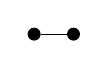
\begin{tikzpicture}[baseline=-0.5mm]
    \newcommand{\sz}{2.5mm}
    \node (r1) at (-\sz, 0) [blackdot]{};
    \node (r2) at ( \sz, 0) [blackdot]{};
    \draw (r1) -- (r2);
  \end{tikzpicture}
\\
  B_3
  &= -\frac{1}{6} \int [c_1(\vr) + h_0(\vr) t_1(\vr)] \, d\vr \\
  &= -\frac{1}{6} \int [c_1(\vr) + f(\vr) t_1(\vr)] \, d\vr \\
  &= -\frac{1}{3} \int c(\vr) \, d\vr
  = -\frac{1}{3}
  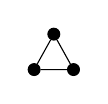
\begin{tikzpicture}[baseline=1.0mm]
    \newcommand{\sz}{2.5mm}
    \node (r1) at (-\sz, 0) [blackdot]{};
    \node (r2) at ( \sz, 0) [blackdot]{};
    \node (r3) at ( 0, 1.8*\sz) [blackdot]{};
    \draw (r1) -- (r2) -- (r3) -- (r1);
  \end{tikzpicture}
\\
  B_4
  &= -\frac{1}{12} \int [c_2(\vr) + h_0(\vr) t_2(\vr) + h_1(\vr) t_1(\vr)] \, d\vr \\
  &= -\frac{1}{12} \int [2 c_2(\vr) + h_1(\vr) t_1(\vr)] \, d\vr \\
  &= -\frac{1}{12} \int \left(
  2 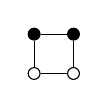
\begin{tikzpicture}[baseline=-1.0mm]
    \newcommand{\sz}{2.5mm}
    \node (r1) at (-\sz, -\sz) [whitedot]{};
    \node (r2) at ( \sz, -\sz) [whitedot]{};
    \node (r3) at ( \sz,  \sz) [blackdot]{};
    \node (r4) at (-\sz,  \sz) [blackdot]{};
    \draw (r1) -- (r2) -- (r3) -- (r4) -- (r1);
  \end{tikzpicture}
  +
  2 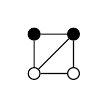
\begin{tikzpicture}[baseline=-1.0mm]
    \newcommand{\sz}{2.5mm}
    \node (r1) at (-\sz, -\sz) [whitedot]{};
    \node (r2) at ( \sz, -\sz) [whitedot]{};
    \node (r3) at ( \sz,  \sz) [blackdot]{};
    \node (r4) at (-\sz,  \sz) [blackdot]{};
    \draw (r1) -- (r2) -- (r3) -- (r4) -- (r1) -- (r3);
  \end{tikzpicture}
  +
  2 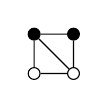
\begin{tikzpicture}[baseline=-1.0mm]
    \newcommand{\sz}{2.5mm}
    \node (r1) at (-\sz, -\sz) [whitedot]{};
    \node (r2) at ( \sz, -\sz) [whitedot]{};
    \node (r3) at ( \sz,  \sz) [blackdot]{};
    \node (r4) at (-\sz,  \sz) [blackdot]{};
    \draw (r1) -- (r2) -- (r3) -- (r4) -- (r1) (r2) -- (r4);
  \end{tikzpicture}
  +
  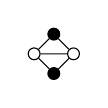
\begin{tikzpicture}[baseline=-1.0mm]
    \newcommand{\sz}{2.5mm}
    \node (r1) at (-\sz, 0) [whitedot]{};
    \node (r2) at ( \sz, 0) [whitedot]{};
    \node (r3) at (   0,  \sz) [blackdot]{};
    \node (r4) at (   0, -\sz) [blackdot]{};
    \draw (r1) -- (r3) -- (r2) -- (r1) -- (r4) -- (r2);
  \end{tikzpicture}
  +
  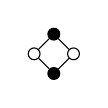
\begin{tikzpicture}[baseline=-1.0mm]
    \newcommand{\sz}{2.5mm}
    \node (r1) at (-\sz, 0) [whitedot]{};
    \node (r2) at ( \sz, 0) [whitedot]{};
    \node (r3) at (   0,  \sz) [blackdot]{};
    \node (r4) at (   0, -\sz) [blackdot]{};
    \draw (r1) -- (r3) -- (r2) (r1) -- (r4) -- (r2);
  \end{tikzpicture}
  \right) \, d \vr
  \notag \\
  &= -\frac{1}{12} \left(
  3 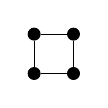
\begin{tikzpicture}[baseline=-1.0mm]
    \newcommand{\sz}{2.5mm}
    \node (r1) at (-\sz, -\sz) [blackdot]{};
    \node (r2) at ( \sz, -\sz) [blackdot]{};
    \node (r3) at ( \sz,  \sz) [blackdot]{};
    \node (r4) at (-\sz,  \sz) [blackdot]{};
    \draw (r1) -- (r2) -- (r3) -- (r4) -- (r1);
  \end{tikzpicture}
  +
  5 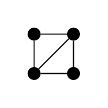
\begin{tikzpicture}[baseline=-1.0mm]
    \newcommand{\sz}{2.5mm}
    \node (r1) at (-\sz, -\sz) [blackdot]{};
    \node (r2) at ( \sz, -\sz) [blackdot]{};
    \node (r3) at ( \sz,  \sz) [blackdot]{};
    \node (r4) at (-\sz,  \sz) [blackdot]{};
    \draw (r1) -- (r2) -- (r3) -- (r4) -- (r1) -- (r3);
  \end{tikzpicture}
  \right)
\end{align*}


So, Eq. (18) gives the exact $B_2$ and $B_3$.
The value of $B_4$, however, differs from
the compressibility-route $B_4^{(c)}$:
\begin{align*}
B_4^{(c)}
  &= -\frac{1}{12} \left(
  3 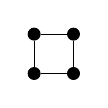
\begin{tikzpicture}[baseline=-1.0mm]
    \newcommand{\sz}{2.5mm}
    \node (r1) at (-\sz, -\sz) [blackdot]{};
    \node (r2) at ( \sz, -\sz) [blackdot]{};
    \node (r3) at ( \sz,  \sz) [blackdot]{};
    \node (r4) at (-\sz,  \sz) [blackdot]{};
    \draw (r1) -- (r2) -- (r3) -- (r4) -- (r1);
  \end{tikzpicture}
  +
  6 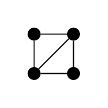
\begin{tikzpicture}[baseline=-1.0mm]
    \newcommand{\sz}{2.5mm}
    \node (r1) at (-\sz, -\sz) [blackdot]{};
    \node (r2) at ( \sz, -\sz) [blackdot]{};
    \node (r3) at ( \sz,  \sz) [blackdot]{};
    \node (r4) at (-\sz,  \sz) [blackdot]{};
    \draw (r1) -- (r2) -- (r3) -- (r4) -- (r1) -- (r3);
  \end{tikzpicture}
  \right)
\end{align*}
%
The difference
$
  -\frac{1}{12}
  \int \left(
  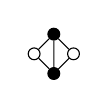
\begin{tikzpicture}[baseline=-1.0mm]
    \newcommand{\sz}{2.5mm}
    \node (r1) at (-\sz, 0) [whitedot]{};
    \node (r2) at ( \sz, 0) [whitedot]{};
    \node (r3) at (   0,  \sz) [blackdot]{};
    \node (r4) at (   0, -\sz) [blackdot]{};
    \draw (r1) -- (r3) -- (r2) (r1) -- (r4) -- (r2) (r3) -- (r4);
  \end{tikzpicture}
  \right) \, d \vr
$
is due to that we have dropped
interface pairs in the derivation (see supplemental material).



\subsection{Shaul et al.'s formula for the cavity function}



First, we have
\begin{align*}
  y(\vr)
  &= \exp t(\vr) \\
  &= \sum_{k = 0}^\infty \frac{1}{k!} \bigl[ t(\vr) \bigr]^k
  = \sum_{k = 0}^\infty \frac{1}{k!} \left[ \sum_{i = 1}^\infty t_i \rho^i \right]^k \\
  &= \sum_{k = 0}^\infty
  \frac{1}{k!}
  \sum_{ (l_1, \dots, l_k) } t_{l_1} \dots t_{l_k}
  \rho^{l_1 + \dots + l_k}
\end{align*}
Taking the $l$th component yields the equation.



\subsection{Derivation of Eq. (20)}



Since
\begin{equation}
  y = y_0 + y_1 \rho + y_2 \rho^2 + \cdots,
  \tag{19}
\label{eq:yrseries}
\end{equation}
we have
\[
  \partial_\rho y = y_1  + 2 y_2 \rho + \cdots
  = \sum_{l = 1}^\infty l y_l \rho^{l-1}.
\]
Similarly, we have
\[
  \partial_\rho t = t_1  + 2 t_2 \rho + \cdots
  = \sum_{j = 1}^\infty j t_j \rho^{j-1}.
\]
Plug them into $\partial_\rho y = y \, \partial_\rho t$,
we get
\begin{align*}
  \sum_{l = 1}^\infty l y_l \rho^{l - 1}
&= \sum_{i = 0}^\infty y_i \rho^i
  \sum_{j = 1}^\infty j t_j \rho^{j - 1},
  \quad \mbox{(set $i \rightarrow l - j$)}
  \\
&=
  \sum_{l = 1}^\infty
  \left(
  \sum_{j = 1}^l y_{l - j} j t_j
  \right) \rho^{l - 1}.
\end{align*}
Then take the coefficient before $\rho^{l-1}$, and
\begin{equation}
  y_l = \frac{1}{l} \sum_{j = 1}^l y_{l - j} \, j \, t_j.
  \tag{20}
  \label{eq:ylexpseries}
\end{equation}



\subsection{Pressure and chemical potential}



From the first law,
\[
  dE = T dS - P dV + \mu dN.
\]
So,
\[
  -\left. \frac{ \partial P } {\partial N} \right|_{V}
  = \left. \frac{ \partial \mu } { \partial V } \right|_{N}.
\]
It follows,
\[
  -\left. \frac{ \partial P } {V \, \partial \rho} \right|_{V}
  = \left. \frac{ \partial \mu } {N \, \partial (1/\rho) } \right|_{N}.
\]
So
\begin{equation}
  \frac{ \partial P } {\rho \, \partial \rho}
  = \frac{ \partial \mu } { \partial \rho }.
  \label{eq:Pmu}
\end{equation}

For the excess part
\begin{equation}
  \frac{ \partial  \Pex } {\rho \, \partial \rho}
  = \frac{ \partial \muex } { \partial \rho }.
  \label{eq:Pmu}
\end{equation}

We now expand
\begin{equation}
  -\beta \muex = \sum_{n = 2}^\infty \beta_{n-1} \rho^{n-1}.
  \label{eq:expandmu}
\end{equation}
Then
\[
  \sum_{n = 2}^\infty n B_n \rho^{n-2}
=
  -\sum_{n = 2}^\infty \beta_{n-1} \rho^{n-2},
\]
which means
\begin{equation}
  B_n = \frac{1-n}{n}\beta_{n-1}.
  \label{eq:Bbeta}
\end{equation}



\subsection{Chemical potential for the HNC closure}



The formula is
\begin{equation}
  -\beta \muex = \rho \int \left( c - \tfrac{1}{2} h \, t\right) d\vr.
  \label{eq:muex}
\end{equation}

To show this,
we start from differentiating $g = (1+f)y$ with respect to
the charging parameters $\xi$.
The charging parameter affects only the potential terms involving
the designated particle 1;
$\xi = 0$ means particle 1 is not interacting with the rest of the particles,
$\xi = 1$ means particle 1 is identical to any other particle:
\begin{align*}
  \partial_\xi g
  &= (\partial_\xi f) \, y + (1+f) \, \partial_\xi y
  = (\partial_\xi f) \, y + (1+f) \, y \, \partial_\xi t \\
  &= (\partial_\xi f) \, y + g \, \partial_\xi t,
\end{align*}
Here, we have used $y = \exp t$ so that $\partial_\xi y = y \, \partial_\xi t$.

Next, we will use
\begin{align*}
  -\beta \muex
  = \rho \int_0^1 d\xi \int_\vr (\partial_\xi f) \, y \, d\vr \\
\end{align*}
where factor $\rho$ comes about because
\[
   N \, (N - 1)
=
  \int_{\vr'} \int_\vr \rho(\vr, \vr') \, d\vr \, d\vr'
=
  \rho^2 \int_{\vr'}  \int_\vr g(\vr, \vr') \, d\vr \, d\vr'
=
  \rho \, N \int_\vr g(\vr) \, d\vr,
\]
Thus,
\[
  N - 1
  = \rho \int_\vr g \, d\vr
  = \rho \int_\vr f \, y \, d \vr,
\]
which gives the number of particles interacting with particle 1.
%
Then,
\begin{align*}
  -\beta \muex
  &= \rho \int_0^1 d\xi \int d\vr \, (\partial_\xi g - g \, \partial_\xi t) \\
  &= \rho \int_0^1 d\xi \int d\vr \, (\partial_\xi c - h \, \partial_\xi t) \\
  &= \rho \int_0^1 d\xi \int d\vr \, \partial_\xi \left(c - \tfrac{1}{2} h \, t \right) \\
  &= \rho \int d\vr \, \left(c - \tfrac{1}{2} h \, t \right).
\end{align*}
We have assumed infinite dilution on the third line so that
$t \, \partial_\xi h = h \, \partial_\xi t = \tfrac{1}{2} \partial_\xi (h t)$.


Now for the virial coefficients,
using \eqref{eq:expandmu},
we get
%\begin{multline*}
\[
  \sum_{n = 2}^\infty \beta_{n - 1} \rho^{n - 1}
%\\
= \rho \int
  \left[
  \sum_{l = 0}^\infty c_l \, \rho^l
  -\frac{1}{2}
  \sum_{l = 1}^\infty
  \left(
  \sum_{j = 1}^l h_{l - j} t_j
  \right) \rho^l
  \right] d\vr.
\]
%\end{multline*}
Setting $l = n - 2$, we get
\[
  \beta_{n - 1}
= \int_\vr
  \left(
    c_{n-2}
  -\frac{1}{2}
  \sum_{j = 1}^{n-2} h_{n - 2 - j} t_j
  \right) \, d\vr.
\]
By using \eqref{eq:Bbeta},
\[
  B_n
= \frac{1-n}{n} \int_\vr
  \left(
    c_{n-2}
  -\frac{1}{2}
  \sum_{j = 1}^{n-2} h_{n - 2 - j} t_j
  \right) \, d\vr.
\]

A few special cases are given below
\begin{align*}
  B_2
  &= -\frac{1}{2} \int c_0(\vr) \, d\vr
  = -\frac{1}{2} \int f(\vr) \, d\vr
  = -\frac{1}{2}
  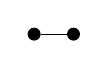
\begin{tikzpicture}[baseline=-0.5mm]
    \newcommand{\sz}{2.5mm}
    \node (r1) at (-\sz, 0) [blackdot]{};
    \node (r2) at ( \sz, 0) [blackdot]{};
    \draw (r1) -- (r2);
  \end{tikzpicture}
\\
  B_3
  &= -\frac{2}{3} \int \left[ c_1(\vr) - \frac{1}{2} h_0(\vr) t_1(\vr) \right] \, d\vr \\
  &= -\frac{2}{3} \int \left[ c_1(\vr) - \frac{1}{2} f(\vr) t_1(\vr) \right] \, d\vr \\
  &= -\frac{1}{3} \int c(\vr) \, d\vr
  = -\frac{1}{3}
  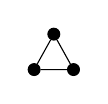
\begin{tikzpicture}[baseline=1.0mm]
    \newcommand{\sz}{2.5mm}
    \node (r1) at (-\sz, 0) [blackdot]{};
    \node (r2) at ( \sz, 0) [blackdot]{};
    \node (r3) at ( 0, 1.8*\sz) [blackdot]{};
    \draw (r1) -- (r2) -- (r3) -- (r1);
  \end{tikzpicture}
\\
  B_4
  &= -\frac{3}{4} \int \left[c_2(\vr) - \frac{1}{2} h_0(\vr) t_2(\vr) -\frac{1}{2} h_1(\vr) t_1(\vr)\right] \, d\vr \\
  &= -\frac{3}{4} \int \left[
      \frac{1}{2} f(\vr) t_2(\vr)
    + \frac{1}{2} h_1(\vr) t_1(\vr)
    - \frac{1}{2} h_1(\vr) t_1(\vr) \right] \, d\vr \\
  &= -\frac{3}{8} \int
      f(\vr) t_2(\vr) \, d\vr \\
  &= -\frac{3}{8} \int \left(
  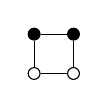
\begin{tikzpicture}[baseline=-1.0mm]
    \newcommand{\sz}{2.5mm}
    \node (r1) at (-\sz, -\sz) [whitedot]{};
    \node (r2) at ( \sz, -\sz) [whitedot]{};
    \node (r3) at ( \sz,  \sz) [blackdot]{};
    \node (r4) at (-\sz,  \sz) [blackdot]{};
    \draw (r1) -- (r2) -- (r3) -- (r4) -- (r1);
  \end{tikzpicture}
  +
  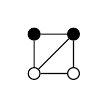
\begin{tikzpicture}[baseline=-1.0mm]
    \newcommand{\sz}{2.5mm}
    \node (r1) at (-\sz, -\sz) [whitedot]{};
    \node (r2) at ( \sz, -\sz) [whitedot]{};
    \node (r3) at ( \sz,  \sz) [blackdot]{};
    \node (r4) at (-\sz,  \sz) [blackdot]{};
    \draw (r1) -- (r2) -- (r3) -- (r4) -- (r1) -- (r3);
  \end{tikzpicture}
  +
  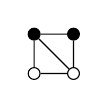
\begin{tikzpicture}[baseline=-1.0mm]
    \newcommand{\sz}{2.5mm}
    \node (r1) at (-\sz, -\sz) [whitedot]{};
    \node (r2) at ( \sz, -\sz) [whitedot]{};
    \node (r3) at ( \sz,  \sz) [blackdot]{};
    \node (r4) at (-\sz,  \sz) [blackdot]{};
    \draw (r1) -- (r2) -- (r3) -- (r4) -- (r1) (r2) -- (r4);
  \end{tikzpicture}
  \right) \, d \vr
  \notag \\
  &= -\frac{3}{8}
  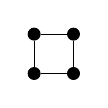
\begin{tikzpicture}[baseline=-1.0mm]
    \newcommand{\sz}{2.5mm}
    \node (r1) at (-\sz, -\sz) [blackdot]{};
    \node (r2) at ( \sz, -\sz) [blackdot]{};
    \node (r3) at ( \sz,  \sz) [blackdot]{};
    \node (r4) at (-\sz,  \sz) [blackdot]{};
    \draw (r1) -- (r2) -- (r3) -- (r4) -- (r1);
  \end{tikzpicture}
  - \frac{3}{4}
  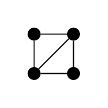
\begin{tikzpicture}[baseline=-1.0mm]
    \newcommand{\sz}{2.5mm}
    \node (r1) at (-\sz, -\sz) [blackdot]{};
    \node (r2) at ( \sz, -\sz) [blackdot]{};
    \node (r3) at ( \sz,  \sz) [blackdot]{};
    \node (r4) at (-\sz,  \sz) [blackdot]{};
    \draw (r1) -- (r2) -- (r3) -- (r4) -- (r1) -- (r3);
  \end{tikzpicture}.
\end{align*}
%
The above examples shows that the virial coefficients
are identical to the virial-route results.



\subsection{Eq. (21)}



Diagrammatically, $\log y$ collects all diagrams
such that the two roots are nonadjacent
and they do not form an articulation pair.
%
Thus, if $\log y(\vr)$ is exactly expanded, we have
\[
  \log y(\vr)
  =
  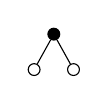
\begin{tikzpicture}[baseline=-1.0mm]
    \newcommand{\sz}{2.5mm}
    \node (r1) at (-\sz, -\sz) [whitedot]{};
    \node (r2) at ( \sz, -\sz) [whitedot]{};
    \node (r3) at ( 0,  0.8*\sz) [blackdot]{};
    \draw (r2) -- (r3) -- (r1);
  \end{tikzpicture}
  +
  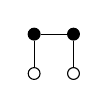
\begin{tikzpicture}[baseline=-1.0mm]
    \newcommand{\sz}{2.5mm}
    \node (r1) at (-\sz, -\sz) [whitedot]{};
    \node (r2) at ( \sz, -\sz) [whitedot]{};
    \node (r3) at ( \sz,  \sz) [blackdot]{};
    \node (r4) at (-\sz,  \sz) [blackdot]{};
    \draw (r2) -- (r3) -- (r4) -- (r1);
  \end{tikzpicture}
  +
  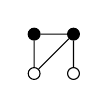
\begin{tikzpicture}[baseline=-1.0mm]
    \newcommand{\sz}{2.5mm}
    \node (r1) at (-\sz, -\sz) [whitedot]{};
    \node (r2) at ( \sz, -\sz) [whitedot]{};
    \node (r3) at ( \sz,  \sz) [blackdot]{};
    \node (r4) at (-\sz,  \sz) [blackdot]{};
    \draw (r2) -- (r3) -- (r4) -- (r1) (r1) -- (r3);
  \end{tikzpicture}
  +
  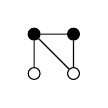
\begin{tikzpicture}[baseline=-1.0mm]
    \newcommand{\sz}{2.5mm}
    \node (r1) at (-\sz, -\sz) [whitedot]{};
    \node (r2) at ( \sz, -\sz) [whitedot]{};
    \node (r3) at ( \sz,  \sz) [blackdot]{};
    \node (r4) at (-\sz,  \sz) [blackdot]{};
    \draw (r2) -- (r3) -- (r4) -- (r1) (r2) -- (r4);
  \end{tikzpicture}
  +
  \frac{1}{2}
  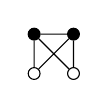
\begin{tikzpicture}[baseline=-1.0mm]
    \newcommand{\sz}{2.5mm}
    \node (r1) at (-\sz, -\sz) [whitedot]{};
    \node (r2) at ( \sz, -\sz) [whitedot]{};
    \node (r3) at ( \sz,  \sz) [blackdot]{};
    \node (r4) at (-\sz,  \sz) [blackdot]{};
    \draw (r2) -- (r3) -- (r4) -- (r1) (r2) -- (r4) (r1) -- (r3);
  \end{tikzpicture}
  + \cdots
\]

At zero separation,
\[
  \log y(\vct 0)
  =
  - \,
  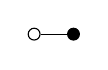
\begin{tikzpicture}[baseline=-3.5mm]
    \newcommand{\sz}{2.5mm}
    \node (r1) at (-\sz, -\sz) [whitedot]{};
    \node (r2) at ( \sz, -\sz) [blackdot]{};
    \draw (r1) -- (r2);
  \end{tikzpicture}
  -\frac{1}{2} \,
  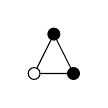
\begin{tikzpicture}[baseline=-1.0mm]
    \newcommand{\sz}{2.5mm}
    \node (r1) at (-\sz, -\sz) [whitedot]{};
    \node (r2) at ( \sz, -\sz) [blackdot]{};
    \node (r3) at (   0,  \sz) [blackdot]{};
    \draw (r1) -- (r2) -- (r3) -- (r1);
  \end{tikzpicture}
  - \cdots
\]

Therefore,
%
\begin{align*}
  B_2
  &= -\frac{1}{2} \,
  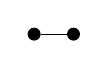
\begin{tikzpicture}[baseline=-0.5mm]
    \newcommand{\sz}{2.5mm}
    \node (r1) at (-\sz, 0) [blackdot]{};
    \node (r2) at ( \sz, 0) [blackdot]{};
    \draw (r1) -- (r2);
  \end{tikzpicture}
\\
  B_3
  &= -\frac{1}{3} \,
  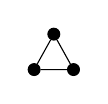
\begin{tikzpicture}[baseline=1.0mm]
    \newcommand{\sz}{2.5mm}
    \node (r1) at (-\sz, 0) [blackdot]{};
    \node (r2) at ( \sz, 0) [blackdot]{};
    \node (r3) at ( 0, 1.8*\sz) [blackdot]{};
    \draw (r1) -- (r2) -- (r3) -- (r1);
  \end{tikzpicture},
  \dots
\end{align*}
%
which are both correct.



\subsection{Eq. (26)}



For $l \ge 1$, the compressibility- and virial- route
results are given by
\begin{align*}
  B^{(c)}_n
&=
  -\frac{1}{n} \int c_{n-2}(\vr) \, d\vr
\\
&=
-\frac{1}{n}
\int \Big[
  f \, t_{n-2} + \lambda_{n-2} \, (1+ f) \, w_{n-2}
\Big] \, d\vr
\\
&=B^{(c, \mathrm{uncorr})}_n
 + \lambda_{n-2} \, \Delta B^{(c)}_n
\end{align*}
and
\begin{align*}
  B^{(v)}_n
&=
  \frac{1}{2D} \int rf' \, y_{n-2} \, d\vr
\\
&=
\frac{1}{2D} \int rf'\, (t_{n-2} + \lambda_{n-2} w_{n-2}) \, d\vr
\\
&=B^{(v, \mathrm{uncorr})}_n
 + \lambda_{n-2} \, \Delta B^{(v)}_n
\end{align*}

To make the two equal
\[
\lambda_{n-2} \left[ \Delta B^{(c)}_n - \Delta B^{(v)}_n \right]
  = B^{(v, \mathrm{uncorr})}_n
  - B^{(c, \mathrm{uncorr})}_n,
\]
which leads to Eq. (26).




\section{Main text: Results}



%\subsection{Geometric closure}
%
%The closure
%\begin{align*}
%  y
%&=
%1 + t/(1 - \eta \, t/2)
%\\
%&=
%1 + t  + \eta t^2/2 + \eta^2 t^3/4 + \eta^3 t^4/8 + \cdots
%\end{align*}
%
%
%
%\subsection{Logarithmic closure}
%
%The closure
%\begin{align*}
%  y
%&=
%1 - \log(1 - \eta t)/\eta
%\\
%&=
%1 + t  + \eta t^2/2 + \eta^2 t^3/3 + \eta^3 t^4/4 + \cdots
%\end{align*}



\subsection{Table II}


Table \ref{tab:reprod_TableII}
shows how to reproduce Table II of the main text.
%
The source code,
\texttt{ievir.c}, \texttt{ybgvir.c}, and \texttt{kirkvir.c}, etc.,
is located under the directory
\texttt{prog/ie}.
%
For each row of the table,
we recompile the corresponding source code
and run the listed command.
%
No extrapolation is needed for the presented precision.
%
We used \texttt{long double},
and \texttt{\_\_float128} appears to be unnecessary.
%

\begin{table}\footnotesize
  \begin{tabular}{p{3cm} p{11cm} p{2cm}}
  Closure
  &
  Command
  &
  Notes \\
  \hline
  YBG
  &
  \texttt{
    gcc -O3 -Wall -DLDBL ybgvir.c -lfftw3l -lm
    \newline
    \&\& ./a.out -n 14 -M 1048576
  }
  &
  \\
  Kirkwood
  &
  \texttt{
    gcc -O3 -Wall -DLDBL kirkvir.c -lfftw3l -lm
    \newline
    \&\& ./a.out -n 14 -M 1048576
  }
  &
  \\
  PY
  &
  \texttt{
    gcc -O3 -Wall -DLDBL -DFFTW ievir.c -lfftw3l -lm
    \newline
    \&\& ./a.out -n 14 -M 4194304
  }
  &
  \\
  HNC
  &
  \texttt{
    gcc -O3 -Wall -DLDBL -DFFTW ievir.c -lfftw3l -lm
    \newline
    \&\& ./a.out -n 14 -M 4194304 --hnc
  }
  &
  \\
  Hurst, \newline
    $m = 0.41718$
  &
  \texttt{
    gcc -O3 -Wall -DLDBL -DFFTW ievir.c -lfftw3l -lm
    \newline
    \&\& ./a.out -n 14 -M 4194304 --hm 0.41718
  }
  &
  \\
  Rowlinson 1, \newline
    $\eta = 0.16564$
  &
  \texttt{
    gcc -O3 -Wall -DLDBL -DFFTW ievir.c -lfftw3l -lm
    \newline
    \&\& ./a.out -n 14 -M 8388608 --rphi 0.16564
  }
  &
  \\
  Rowlinson 2, \newline
    $\eta = 0.16564$
  &
  \texttt{
    gcc -O3 -Wall -DLDBL -DFFTW ievir.c -lfftw3l -lm
    \newline
    \&\& ./a.out -n 14 -M 8388608 --iphi 0.16564
  }
  &
  \\
  HC, \newline
    $s = 0.83436$
  &
  \texttt{
    gcc -O3 -Wall -DLDBL -DFFTW ievir.c -lfftw3l -lm
    \newline
    \&\& ./a.out -n 14 -M 8388608 --hcs 0.83436
  }
  &
  \\
  MS
  &
  \texttt{
    gcc -O3 -Wall -DLDBL -DFFTW ievir.c -lfftw3l -lm
    \newline
    \&\& ./a.out -n 14 -M 8388608 --ms
  }
  &
  \\
  BPGG, \newline
  $s = 1.83436$
  &
  \texttt{
    gcc -O3 -Wall -DLDBL -DFFTW ievir.c -lfftw3l -lm
    \newline
    \&\& ./a.out -n 14 -M 8388608 --bpggs 1.83436
  }
  &
  \\
  Verlet, \newline
  $A = 0.83436$, \newline
  $B = 1.54751$
  &
  \texttt{
    gcc -O3 -Wall -DLDBL -DFFTW ievir.c -lfftw3l -lm
    \newline
    \&\& ./a.out -n 14 -M 8388608 --va 0.83436 --vb 1.54751
  }
  &
  \\
  MP, \newline
  $\eta = 0.16564$
  &
  \texttt{
    gcc -O3 -Wall -DLDBL -DFFTW ievir.c -lfftw3l -lm
    \newline
    \&\& ./a.out -n 14 -M 8388608 -q 0.16564
  }
  &
  \\
  RY, \newline
  $\alpha = 0.17015$
  &
  \texttt{
    gcc -O3 -Wall -DLDBL -DFFTW ievir.c -lfftw3l -lm
    \newline
    \&\& ./a.out -n 14 -M 8388608 --rya 0.17015
  }
  &
  \\
  Square, \newline
  $\alpha = 0.16564$
  &
  \texttt{
    gcc -O3 -Wall -DLDBL -DFFTW ievir.c -lfftw3l -lm
    \newline
    \&\& ./a.out -n 14 -M 8388608 --sqrs 0.16564
  }
  &
  \\
  \hline
  \end{tabular}
  \caption{
    \label{tab:reprod_TableII}
    Reproduction of Table II in the main text.
  }
\end{table}



\subsection{Table V}



\subsubsection{Reference values}



To reproduce the reference value (last value) of
each cell in Table V,
first go to the directory
\texttt{data/gaussf}.
For each cell, $D_n$,
run the command

\qquad\texttt{python gaussfextra.py D n}

For example, for the cell $8_{13}$,
run

\qquad\texttt{python gaussfextra.py 8 13}



\section{Appendix A.1: Fourier transforms in odd dimensions}



\subsection{Basics of the Bessel function}



A relatively easy way to remember the Bessel function
is through the generating function
%
\begin{equation}
  g(z, t)
  =
  \exp\left[ \frac{z}{2} \left(t - \frac{1}{t}\right) \right]
  =
  \sum_{\nu = \infty}^\infty J_\nu(z) \, t^\nu.
  \label{eq:BesselGF}
\end{equation}
%
Expanding the left side yields
\begin{align*}
&
  \sum_{l = 0}^\infty \frac{ 1 } { l! } \left( \frac {z \, t} 2\right)^l
  \sum_{s = 0}^\infty \frac{ (-)^s } { s! }
    \left( \frac z {2t} \right)^s
  \quad \mbox{(set $l \rightarrow s + \nu$)} \\
&=
  \sum_{\nu = -\infty}^\infty
  \left[
  \sum_{s = 0}^\infty
  \frac { (-)^s } {s! (\nu + s)! }
  \left( \frac z 2 \right)^{\nu + 2s}
  \right]
  \, t^\nu
\end{align*}
So,
\begin{equation}
  J_\nu(z)
=
  \sum_{s = 0}^\infty
  \frac{ (-)^s } { s! (\nu + s)! }
  \left( \frac z 2 \right)^{\nu + 2s}.
  \label{eq:bessel}
\end{equation}



\subsection{Recurrence relations of the Bessel function}

Several recurrence relations can be derived from the generating function,
Eq. \eqref{eq:BesselGF}, which we will use later on.

First,
\begin{equation}
  \frac { \partial g } { \partial z}
+
  \frac { t \partial g } { z \partial t}
=
  t g.
  \label{eq:BesselR1g}
\end{equation}
or
\[
\frac 1 2 \left( t - \frac 1 t \right) \, g
+
\frac {t} {2 z} \left( 1 + \frac 1 { t^2 } \right) \, g
=
  t \, g.
\]

Now expanding both sides of Eq. \eqref{eq:BesselR1g},
we get
\[
  \sum_\nu J'_\nu(z) \, t^\nu
+
  \sum_\nu \frac{ \nu \, J_\nu(z) } { z } t^\nu
=
  \sum_\nu J_{\nu}(z) \, t^{\nu+1},
\]
or
\[
  J'_\nu(z)
+
  \frac{ \nu \, J_\nu(z) } { z }
=
  J_{\nu - 1}(z),
\]
which can be written as
\begin{align}
  \frac{d}{dz} [z^{\nu} J_\nu(z)] = z^{\nu} J_{\nu-1}(z),
  \label{eq:BesselR1}
\end{align}

Similarly, from
\begin{equation}
-
  \frac { \partial g } { \partial z}
+
  \frac { t \partial g } { z \partial t}
=
  \frac{1}{t} \, g,
  \label{eq:BesselR2g}
\end{equation}
we get
\begin{align}
  \frac{d}{dz} [z^{-\nu} J_\nu(z)] = -z^{-\nu} J_{\nu+1}(z),
  \label{eq:BesselR2}
\end{align}





\subsection{Proof of Eq. \eqref{eq:FTsphr}}

The Fourier transform of an isotropic function in $D$ dimensions
is given by
\begin{align}
  \tilde A(k)
&=
\frac{(2\pi)^{D/2}}{k^{D/2-1}}
\int_0^\infty
A(r) \, J_{D/2-1}(kr) \,
r^{D/2} \, dr.
\tag{A1}
\label{eq:FTsphr}
\end{align}

To show Eq. \eqref{eq:FTsphr}, we start with
%
\begin{align}
  \tilde A(k)
&=
  \int_0^\infty
  \int_0^\pi
  A(r) \, \exp(-ikr \cos \theta_D) \,
    r^{D-1} \, dr \,
    \sin^{D-2} \theta_D \,
    d\theta_D \, S_{D-1}(1),
\label{eq:Aksphr}
\end{align}
%
where,
$\theta_D$ is angle between vectors $\vk$ and $\vr$,
and
$S_{D-1}(1)$ comes from integrating over other angular variables,
Eq. \eqref{eq:SDintang}:
\[
  S_{D-1}(1)
=
\int_0^\pi \sin^{D-3} \theta_{D-1} d\theta_{D-1} \,
\cdots \,
\int_0^\pi \sin \theta_3 d\theta_3 \,
\int_0^{2\pi} d\theta_2
=
\frac{2 \, \pi^{(D-1)/2} } { \Gamma\left( \frac{D-1} 2 \right) }.
\]
%

To evaluate \eqref{eq:Aksphr},
we will use the following identity
\begin{equation}
  \int_0^\pi
  \exp(-iz\cos\theta) \,
  \sin^{2\nu} \theta \,
  d \theta
=
  \frac{ \nu! }{ (z/2)^\nu } \,
  I_{2 \nu} \, J_\nu(z),
  \label{eq:intexpsin}
\end{equation}
%
where $\nu = (D - 2)/2$,
and
\begin{equation}
  I_{2\nu}
=
  I_{D-2}
\equiv
  \int_0^\infty \sin^{D-2} \theta \, d\theta
=
\frac{ S_{D}(1) }
  { S_{D-1}(1) }.
\end{equation}

Thus, \eqref{eq:Aksphr} gives
\begin{align*}
  \tilde A(k)
&=
\int_0^\infty
A(r)
\frac{ \nu! } { (kr/2)^{\nu} } \, J_\nu(kr) \,
S_D(1) \, r^{D-1} \, dr
\\
&=
\int_0^\infty
A(r)
\frac{ \nu! } { (kr/2)^{\nu} } \, J_\nu(kr) \,
\frac{ 2 \pi^{\nu+1} }{ \Gamma(\nu+1) }
\, r^{2\nu+1} \, dr
\\
&=
\frac{(2\pi)^{\nu+1}}{k^{\nu}}
\int_0^\infty
A(r) \, J_\nu(kr) \,
r^{\nu+1} \, dr.
\end{align*}
which is Eq. \eqref{eq:FTsphr} upon $\nu \rightarrow D/2-1$.



\subsection{Proof of Eq. \eqref{eq:intexpsin} }



We now prove Eq. \eqref{eq:intexpsin}.
%
First, it is readily seen that
the imaginary part of the integral is zero
for the integral over $(0, \pi/2)$
is canceled by that over $(\pi/2, \pi)$.
%
Thus, we will show that
\begin{equation}
  \int_0^\pi
  \cos(z\cos\theta) \,
  \sin^{2\nu} \theta \,
  d \theta
=
  \frac{ \nu! }{ (z/2)^\nu } \,
  I_{2 \nu} \, J_\nu(z),
  \label{eq:intccossin}
\end{equation}

Next, the left hand side can be expanded as
%
\begin{align*}
& \;
  \sum_{s = 0}^\infty
  \frac{ (-)^s z^{2s} } { (2s)! }
  \,
  2 \, \int_0^{\pi/2} \cos^{2s} \theta \, \sin^{2\nu} \theta d \theta
  \\
&=
  \sum_{s = 0}^\infty
  \frac{ (-)^s z^{2s} } { (2s)! }
  B(s+\tfrac 1 2, \nu + \tfrac 1 2)
  \\
&=
  \sum_{s = 0}^\infty
  \frac{ (-)^s z^{2s} } { (2s)! }
  \frac{ (s-\tfrac 1 2)! (\nu - \tfrac 1 2)! }
       {  (s + \nu)!    }
  \\
&=
  \frac{1}{z^\nu}
  \sum_{s = 0}^\infty
  \frac{ (-)^s z^{2s + \nu} } { (2s)! }
  \frac{ (2s-1)!! \, (\tfrac 1 2)! (\nu - \tfrac 1 2)! }
      { 2^s \, (s + \nu)!    }
\\
&=
  \frac{\nu!}{(z/2)^\nu}
  \sum_{s = 0}^\infty
  \frac{ (-)^s (z/2)^{2s + \nu} } { s! \, (s + \nu)! }
  \frac{ (\tfrac 1 2)! (\nu - \tfrac 1 2)! }
       { \nu!    }
=
\frac{\nu!}{(z/2)^\nu} \, J_\nu(z) \, I_{2\nu}
\end{align*}
Here, we have used the doubling formula:
\begin{equation}
  (s - \tfrac 1 2)! = \sqrt\pi \, (2 s - 1)!! / 2^s
\end{equation}
and
\[
  I_{2\nu}
=
B(\nu + \tfrac{1}{2}, \tfrac{1}{2})
=
\frac{ (\tfrac 1 2)! (\nu - \tfrac 1 2)! }
       { \nu!    }.
\]



\subsection{Small $k$ limit of Eq. \eqref{eq:FTsphr}}



One way to convince yourself of Eq. \eqref{eq:FTsphr} is to study the small $k$ limit.
%
Keeping the first term in \eqref{eq:bessel} yields
\[
  J_\nu(z) \rightarrow \frac{ (z/2)^\nu }{ \nu! }
\]
So
%
\begin{align*}
\tilde A(k \rightarrow 0)
&\approx
\frac{ (2 \pi)^{D/2} } { k^{D/2 - 1} \Gamma(D/2) }
\int_0^\infty A(r) \, \left( \frac{k r}{2} \right)^{D/2 - 1} dr \\
&=
\frac{ 2 \pi^{D/2} } { \Gamma(D/2) }
\int_0^\infty A(r) \, r^{D/2 - 1} dr.
\end{align*}
%
The pre-factor is indeed the surface area
given by \eqref{eq:surfareaD}.


The inverse of Eq. \eqref{eq:FTsphr} is
\begin{equation}
A(r)
=
\frac{ (2\pi)^{-D/2} } { r^{D/2 - 1} }
\int_0^\infty \tilde{A}(k) \, J_{D/2-1}(kr) \, k^{D/2} \, dk.
\label{eq:invFTsphr}
\end{equation}
Note that, besides $k \leftrightarrow r$,
the $(2\pi)^{D/2}$ in the pre-factor is now $(2\pi)^{-D/2}$
for we have to divide the result by $(2\pi)^D$
for the inverse Fourier transform.



\subsection{Eq. (A2)}

Since $D = 2\delta + 3$, $D/2 - 1 = \delta + 1/2$.
%
Next $J_{D/2-1}(kr) \rightarrow \sqrt{2 k r/\pi} j_{D/2-3/2} (kr)$.
%
So
\begin{align*}
\tilde A(k)
&=
\frac{ (2 \pi)^{\delta + 3/2} } { k^{\delta + 1/2} }
\int_0^R
  A(r) \, \frac{ (2kr)^{1/2} } { \pi^{1/2} } \,
  j_\delta(k r) \, r^{\delta + 3/2}\, dr \\
&=
  \frac{ 2^{\delta + 2} \pi^{\delta + 1} } { k^\delta }
\int_0^R
  A(r) \, j_\delta(k r) \, r^{\delta + 2} \, dr.
\end{align*}



\subsection{Spherical Bessel functions}

The following formula is deleted from version 5 of the manuscript
\begin{equation}
  j_\delta(x)
=
  (-x)^\delta \,
  \left(
    \frac{ d }
    { x \, dx }
  \right)^\delta
  \,
  \left(
    \frac{ \sin x } { x }
  \right).
\end{equation}
This formula can be readily used to expand
spherical Bessel functions
as rational combinations of $\sin x$ and $\cos x$.

The first few spherical Bessel functions are
\begin{align*}
  j_0(x)
&=
  \frac{ \sin(x) } { x },
\\
  j_1(x)
&=
  \frac{ \sin(x) } { x^2 }
-
  \frac{ \cos(x) } { x },
\\
  j_2(x)
&=
  \left(
    \frac{ 3 } { x^3 }
    -
    \frac{ 1 } { x }
  \right)
  \,
  \sin x
  -
  \frac{ 3 } { x^2 }
  \,
  \cos x.
\end{align*}



\section{Appendix A.2: Fourier transforms in even dimensions}

\subsection{Hankel transform}

Rewrite Eq. \eqref{eq:FTsphr} as
\[
\tilde{A}(k) \, k^{D/2-1}
= (2 \pi)^{D/2}
\int_0^\infty A(r) \, r^{D/2-1} \, J_{D/2-1}(kr) \, r \, dr.
\]

Now replace $D/2 - 1$ by $\nu$, and
\[
\tilde{A}(k) \, k^\nu
= (2 \pi)^{\nu+1}
\int_0^\infty A(r) \, r^\nu \, J_{\nu}(kr) \, r \, dr.
\]

We now do the following replacements:
\begin{equation}
\begin{split}
  A(r) \, r^\nu \rightarrow \alpha(r) \\
  \tilde{A}(k) \, k^\nu (2\pi)^{-\nu-1}
  \rightarrow
  \hat a(k),
\end{split}
\label{eq:Atoalpha}
\end{equation}
we get
\begin{equation}
\hat a(k)
=
\int_0^\infty \alpha(r) \, J_\nu(kr) \, r \, dr.
\label{eq:HankelTransform}
\end{equation}

For the inverse, we rewrite \eqref{eq:invFTsphr}
\[
A(r) \, r^{D/2-1}
=
(2\pi)^{-D/2}
\int_0^\infty \tilde{A}(k) \, k^{D/2-1} \, J_{D/2-1}(kr) \, k \, dk.
\]

Replacing $D/2 - 1$ by $\nu$ yields
\[
A(r) \, r^\nu
=
(2\pi)^{-\nu-1}
\int_0^\infty \tilde{A}(k) \, k^\nu \, J_\nu(kr) \, k \, dk.
\]

Using \eqref{eq:Atoalpha} gives
\begin{equation}
\alpha(r)
=
\int_0^\infty \hat \alpha(k) J_\nu(kr) \, k \, dk.
\label{eq:inverseHankelTransform}
\end{equation}

So our transform from $\alpha(r)$ to $\hat\alpha(k)$
should be completely symmetric to the inverse transform
from $\hat\alpha(k)$ to $\alpha(r)$.



\subsection{Fourier-Bessel series}

The discretization of Hankel transform
is related to the Fourier-Bessel series\cite{arfken}.
%
Suppose the function $\alpha(r)$ can be expanded as
%
\begin{align}
\alpha(r) = \sum_{m = 1}^\infty \hat\alpha_m \,
  J_\nu\left(
    \frac{ \gamma_{\nu, m} \, r } { R }
  \right),
  \label{eq:FourierBesselSeries}
\end{align}
%
where $\gamma_{\nu, m}$ is the $m$th zero of $J_\nu$.
%
Then, the coefficients $\hat\alpha_m$ are given by
%
\begin{align}
\hat\alpha_m
=
\frac{ 2 } { R^2 \, \left[ J_{\nu+1}(\gamma_{\nu, m}) \right]^2 }
\int_0^R \alpha(r) \, J_\nu\left(
    \frac{ \gamma_{\nu, m} \, r } { R }
  \right) \, r \, dr.
  \label{eq:FourierBesselSeries_cm}
\end{align}
%
Comparing to \eqref{eq:HankelTransform},
we get
\begin{align}
  \hat\alpha_m
=
  \frac{ 2 } { R^2 \, [J_{\nu + 1}(\gamma_{\nu, m})]^2 }
  \,
  \hat\alpha
  \left(
    \frac{ \gamma_{\nu, m} } { R }
  \right).
  \label{eq:twoalphahats}
\end{align}

The proof is the following.
The Bessel function satisfies the following differential equation
\begin{align*}
  \frac{d}{dz} \left( z \, \frac {d J_\nu}{dz} \right)
  + \left(z - \frac{ \nu^2 } { z } \right) \, J_\nu = 0.
\end{align*}
or
\begin{align*}
  \frac{d}{dr} \left[ r \,
    \frac {d}{dr} J_\nu\left( \frac{ \gamma_{\nu, m} \, r } { R } \right)
  \right]
  + \left(
      \frac{\gamma^2_{\nu, m}}{R^2} \,r - \frac{ \nu^2 } { r }
    \right) \, J_\nu\left( \frac{ \gamma_{\nu, m} \, r } { R } \right) = 0.
\end{align*}
%
We now multiply the above by $J_\nu\left( \gamma_{\nu, n} \, r / R \right)$,
and integrate $r$ from $0$ to $R$, and
\begin{align*}
&
  \left.
 J_\nu\left( \frac{ \gamma_{\nu, n} \, r } { R } \right)
  r \frac {d}{dr}
    J_\nu\left( \frac{ \gamma_{\nu, m} \, r } { R } \right)
\right|_0^{R}
-
  \int_0^R
    \frac {d}{dr} J_\nu\left( \frac{ \gamma_{\nu, m} \, r } { R } \right)
    \frac {d}{dr} J_\nu\left( \frac{ \gamma_{\nu, n} \, r } { R } \right)
  \, r \, dr
\\
&+
\frac{\gamma^2_{\nu, m}}{R^2} \int_0^R
J_\nu\left( \frac{ \gamma_{\nu, m} \, r } { R } \right) \,
J_\nu\left( \frac{ \gamma_{\nu, n} \, r } { R } \right) \, r \, dr
-
\nu^2 \int_0^R
J_\nu\left( \frac{ \gamma_{\nu, m} \, r } { R } \right) \,
J_\nu\left( \frac{ \gamma_{\nu, n} \, r } { R } \right) \, \frac{ dr } { r }
= 0.
\end{align*}
The first term vanishes because $J_\nu\left( \gamma_{\nu, n} \right) = 0$.
%
Now subtract the version with $n$ and $m$ swapped,
we get, for $n \ne m$,
\[\int_0^R
J_\nu\left( \frac{ \gamma_{\nu, m} \, r } { R } \right) \,
J_\nu\left( \frac{ \gamma_{\nu, n} \, r } { R } \right) \, r \, dr
= 0.
\]
This proves the orthogonality of
$J_\nu\left( \gamma_{\nu, m} \, r / R \right)$
and
$J_\nu\left( \gamma_{\nu, n} \, r / R \right)$.

If, however, we set $\gamma_{\nu, n} \rightarrow \gamma_{\nu, m} + \delta\gamma$,
then,
\begin{align*}
  \delta \gamma \,
  \gamma_{\nu, m} \,
  J'_\nu( \gamma_{\nu, m} )
  J'_\nu( \gamma_{\nu, m} )
-
  \frac{ 2 \gamma_{\nu, m} \, \delta \gamma }{R^2} \int_0^R
  J^2_\nu( \gamma_{\nu, m} ) \, r \, dr
= 0.
\end{align*}
Now using the recurrence relation
\[
  J'_{\nu}(z) = n J_\nu(z) / z - J_{\nu + 1}(z),
\]
we get (noting that at $z = \gamma_{\nu, m}$, $J(z) = 0$)
\begin{align*}
  \int_0^R
  J^2_\nu( \gamma_{\nu, m} ) \, r \, dr
=
  \frac{
    \left[ J_{\nu+1}( \gamma_{\nu, m} ) \right]^2 \, R^2
  } { 2 }.
\end{align*}


In summary,
\begin{align}
  \int_0^R
  J_\nu( \gamma_{\nu, n} \, r ) \,
  J_\nu( \gamma_{\nu, m} \, r ) \, r \, dr
=
  \delta_{n, m} \,
  \frac{ \left[ J_{\nu+1}( \gamma_{\nu, m} ) \right]^2 \, R^2 } { 2 }.
  \label{eq:FourierBessel_orthonormal}
\end{align}
which proves \eqref{eq:FourierBesselSeries_cm}.



\subsection{Discrete Hankel transform}



In the appendix,
we give the discrete Hankel transform
\begin{align}
\hat\alpha(k_m)
&=
\hat\alpha\left( \frac{ \gamma_{\nu, m} } { R } \right)
\notag
\\
&=
\int_0^R
\alpha(r) \,
J_\nu\left( \frac{ \gamma_{\nu, m} \, r } { R } \right) \, r \, dr
\notag
\\
&=
\frac{ R^2 } { \gamma^2_{\nu, M} }
\sum_{k = 1}^{M - 1}
\alpha(r_k) \,
J_\nu\left( \frac{ \gamma_{\nu, m} \, r_k } { R } \right)
\frac{ 2 } { \left[ J_{\nu + 1}(\gamma_{\nu, k}) \right]^2 },
\label{eq:discreteHankelTransform}
\end{align}
with
$r_k = \left(\gamma_{\nu, k} / \gamma_{\nu, M}\right) R$.
We shall derive this formula below.


Suppose
\begin{align}
\int_0^R
\alpha(r) \,
J_\nu\left( \frac{ \gamma_{\nu, m} \, r } { R } \right) \, r \, dr
=
\sum_{k = 1}^{M - 1} \beta_k \,
\alpha(r_k) \,
J_\nu\left( \frac{ \gamma_{\nu, m} \, r_k } { R } \right),
\label{eq:DHT_beta}
\end{align}
we wish to determine the coefficients $\beta_k$.


First, by using $J_\nu(\gamma_{\nu, n} \, r)$ as $\alpha(r)$
in \eqref{eq:DHT_beta},
we get from \eqref{eq:FourierBessel_orthonormal} that
\begin{align*}
\sum_{k = 1}^{M - 1}
J_\nu\left( \frac{ \gamma_{\nu, n} \, \gamma_{\nu, k} } { \gamma_{\nu, M} } \right) \,
J_\nu\left( \frac{ \gamma_{\nu, m} \, \gamma_{\nu, k} } { \gamma_{\nu, M} } \right) \,
\beta_k
=
  \delta_{n, m} \,
  \frac{ \left[ J_{\nu+1}( \gamma_{\nu, m} ) \right]^2 \, R^2 } { 2 }.
\end{align*}
By $k \rightarrow m$, $m \rightarrow k$, $n \rightarrow k'$, we get
\begin{align}
\sum_{m = 1}^{M - 1}
J_\nu\left( \frac{ \gamma_{\nu, k} \, \gamma_{\nu, m} } { \gamma_{\nu, M} } \right) \,
J_\nu\left( \frac{ \gamma_{\nu, k'} \, \gamma_{\nu, m} } { \gamma_{\nu, M} } \right) \,
\beta_m
=
  \delta_{k, k'} \,
  \frac{ \left[ J_{\nu+1}( \gamma_{\nu, k} ) \right]^2 \, R^2 } { 2 }.
  \label{eq:DHT_orthonormal}
\end{align}



On the other hand,
using \eqref{eq:DHT_beta} in \eqref{eq:FourierBesselSeries_cm} yields
\begin{align*}
\hat\alpha_m
=
\frac{ 2 }
{ R^2 \, \left[ J_{\nu + 1}(\gamma_{\nu,m}) \right]^2 }
\sum_{k' = 1}^{M - 1}
\alpha(r_{k'}) \,
J_\nu\left( \frac{ \gamma_{\nu, m} \, \gamma_{\nu, k'} } { \gamma_{\nu, M} } \right)
\, \beta_{k'}.
\end{align*}

Now $\alpha(r_k)$ can be computed from \eqref{eq:FourierBesselSeries}
as
\begin{align*}
\alpha(r_k)
&= \sum_{m = 1}^\infty \hat\alpha_m \,
  J_\nu\left(
    \frac{ \gamma_{\nu, m} \, r_k } { R }
  \right)
\\
&=
  \sum_{k' = 1}^{M - 1}
  \alpha(r_{k'}) \,
  \frac{ \beta_{k'} }
  { R^2 }
  \sum_{m = 1}^{M - 1}
  \frac{ 2 }
  { \left[ J_{\nu + 1}(\gamma_{\nu,m}) \right]^2 }
  J_\nu\left(
    \frac{ \gamma_{\nu, m} \, \gamma_{\nu, k'} } { \gamma_{\nu, M} }
  \right)
  J_\nu\left(
    \frac{ \gamma_{\nu, m} \, \gamma_{\nu, k} } { \gamma_{\nu, M} }
  \right)
\\
&= \sum_{k' = 1}^{M - 1}
  \alpha(r_{k'}) \, \delta_{k, k'}.
\end{align*}
%
Note that we have changed the up limit of the sum from $\infty$ to $k$.
%
Thus, we have,
\begin{align*}
  \sum_{m = 1}^{M - 1}
  \frac{ 2 }
  { \left[ J_{\nu + 1}(\gamma_{\nu,m}) \right]^2 }
  J_\nu\left( \frac{ \gamma_{\nu, m} \, \gamma_{\nu, k'} } { \gamma_{\nu, M} } \right)
  J_\nu\left(
    \frac{ \gamma_{\nu, m} \, \gamma_{\nu, k} } { \gamma_{\nu, M} }
  \right)
  =
  \delta_{k, k'} \frac{ R^2 } { \beta_{k} },
\end{align*}
Compare this result to \eqref{eq:DHT_orthonormal},
we get
\[
  \beta_k
=
\frac{ 2 \, C } { [ J_{\nu + 1}(\gamma_{\nu, k}) ]^2 },
\]
where $C$ is some constant.



\subsubsection*{Determination of the constant $C$}

For a sufficiently large $k$,
we get, from \eqref{eq:DHT_beta},
\begin{align}
  \int_{r_k}^{r_{k+1}}
  r \, dr
\approx
  \beta_k
=
  \frac{ 2 \, C } { [ J_{\nu + 1}(\gamma_{\nu, k}) ]^2 }
  \label{eq:determ_C}
\end{align}

We now use the asymptotic expansion of the Bessel function\cite{arfken}
\begin{equation}
  J_\nu(z)
\approx
  \sqrt{ \frac{ 2 } { \pi \, z } } \,
  \cos\left[
    z - \left(
        n + \frac 1 2
        \right)
        \left(
          \frac \pi 2
        \right)
  \right].
  \label{eq:Bessel_asympt}
\end{equation}
%
which also shows that
%
\begin{equation}
  \gamma_{\nu, k}
\approx
  \left(
    k + \frac 1 2 + \frac{(-1)^n}{4}
  \right)
  \, \pi,
  \label{eq:BesselZero_asympt}
\end{equation}
%
and
%
\begin{equation}
  \Delta \gamma_{\nu, k}
=
  \gamma_{\nu, k + 1} - \gamma_{\nu, k}
\approx
  \pi.
  \label{eq:BesseldZero_asympt}
\end{equation}


Now since $r_k = R \, \left( \gamma_{\nu, k}/\gamma_{\nu, M} \right)$,
the left hand side of \eqref{eq:determ_C} is roughly
\begin{equation}
  r_k \, \Delta r_k
=
  \left( \frac{ R } { \gamma_{\nu, M} } \right)^2
  \gamma_{\nu, k} \, \Delta \gamma_{\nu, k}
=
  \left( \frac{ R } { \gamma_{\nu, M} } \right)^2
  \gamma_{\nu, k} \, \pi.
  \label{eq:determC_lhs}
\end{equation}


On the other hand, from \eqref{eq:Bessel_asympt}, we get
\[
  J_{\nu+1}(\gamma_{\nu, k})
=
  \pm \sqrt{
    \frac{ 2 }
    { \pi \, \gamma_{\nu, k} }
  }.
\]
So, the right hand side of \eqref{eq:determ_C} is equal to
\begin{equation}
  C \, \gamma_{\nu, k} \, \pi.
  \label{eq:determC_rhs}
\end{equation}
Thus, equating \eqref{eq:determC_lhs} and \eqref{eq:determC_rhs} yields
\[
  C = \left( \frac{ R } { \gamma_{\nu, M} } \right)^2,
\]
and
\[
  \beta_k
=
  \frac{ 2 }
  { [ J_{\nu + 1}(\gamma_{\nu, k}) ]^2 }
  \frac{ R^2 }
  { \gamma^2_{\nu, M} }.
\]
This completes the proof of \eqref{eq:discreteHankelTransform}.





\subsection{Inverse discrete Hankel transform}

We now derive the inverse discrete Hankel transform.

Using \eqref{eq:twoalphahats} in \eqref{eq:FourierBesselSeries},
we get
\begin{align*}
  \alpha(r)
=
\sum_{m = 1}^\infty
\frac{ 2 } { R^2 [J_{\nu + 1}(\gamma_{\nu, m})]^2 }
\hat\alpha
  \left(
    \frac{ \gamma_{\nu, m} } { R }
  \right) \,
J_\nu\left(
    \frac{ \gamma_{\nu, m} \, r } { R }
  \right).
\end{align*}
%
We now set $r = r_k$, and define $k_m = \gamma_{\nu, m}/R$.
Then
\begin{align}
  \alpha(r_k)
&=
  \frac{ 1 }{ R^2 }
  \sum_{m = 1}^{M - 1}
    \hat\alpha(k_m) \,
    J_\nu(k_m r_k) \,
    \frac{ 2 }
    { \left[
        J_{\nu+1}(\gamma_{\nu,m})
      \right]^2 }
\notag
\\
&=
  \frac{ k_{\max}^2 }
       { \gamma_{\nu, M}^2 }
  \sum_{m = 1}^{M - 1}
    \hat\alpha(k_m) \,
    J_\nu\left(
      \frac{ \gamma_{\nu, k} \gamma_{\nu, m} }
           { \gamma_{\nu, M} }
    \right) \,
    \frac{ 2 }
    { \left[
        J_{\nu + 1}(\gamma_{\nu, m})
      \right]^2 },
\label{eq:inverseDiscreteHankelTransform}
\end{align}
where
\[
  k_{\max} = \gamma_{\nu, M} / R.
\]
A comparison of \eqref{eq:inverseDiscreteHankelTransform}
and \eqref{eq:discreteHankelTransform}
shows that the inverse discrete Hankel transform
$\hat\alpha(k) \rightarrow \alpha(r)$
assumes the same form as the Hankel transform
$\alpha(r) \rightarrow \hat\alpha(k)$.



\section{Appendix C: Transformation of series}

\subsection{Product}

Given that $c = a \cdot b$, we have
\begin{align*}
  \sum_{l = 0}^{\infty} c_l \, \rho^l
  &=
  \sum_{i = 0}^{\infty} a_i \rho^i
  \sum_{j = 0}^{\infty} b_j \rho^j
  \qquad \mbox{set $i \rightarrow l - j$}
 \notag \\
  &=
  \sum_{l = 0}^{\infty}
  \left(
  \sum_{j = 0}^{l}
    a_{l-j} b_j \right) \rho^l.
\end{align*}

So
\begin{align}
  c_l = \sum_{j = 0}^{l} a_{l-j} b_j.
  \label{eq:product}
\end{align}



\subsection{Quotient}


Because $a = b \cdot d$,
use the product formula \eqref{eq:product}
\begin{align*}
  a_l
  &= \sum_{j = 0}^{l} b_{l-j} d_j
  = \sum_{j = 0}^{l - 1} b_{l - j} d_j + b_0 d_l,
\\
  &= \sum_{i = 1}^{l} b_{i} d_{l - i} + b_0 d_l.
\end{align*}
So
\begin{align*}
  b_0 \, d_l = a_l -\sum_{j = 1}^{l} b_{i} d_{l - i}.
\end{align*}


\subsection{Power}

From $a \, (\partial_\rho p) = \nu p \, (\partial_\rho a)$,
%
\begin{align*}
  \sum_{i = 0} a_i \rho^i
  \sum_{j = 0} j p_j \rho^{j - 1}
&=
  \nu
  \sum_{i = 0} i a_i \rho^{i - 1}
  \sum_{j = 0} p_j \rho^{j},
\end{align*}

So
\begin{align*}
  \sum_{j = 0}^{l-1} a_{l-j} j p_j + a_0 l p_l
&=
  \sum_{j = 0}^{l-1} \nu (l - j) a_{l - j} p_j
\end{align*}

And,
\begin{align*}
  a_0 l p_l
&=
  \sum_{j = 0}^{l-1} [ \nu (l - j) - j] a_{l - j} p_j
\\
&=
  \sum_{j = 0}^{l-1} [ \nu l - (\nu + 1) j] a_{l - j} p_j.
\end{align*}


\subsection{Logarithm}

Start with the exponential formula
\[
  l y_l = \sum_{j = 1}^l j t_j y_{l - j}
  = \sum_{j = 1}^{l - 1} j t_j y_{l - j} + l t_l.
\]
So
\[
  t_l = y_l - \sum_{j = 1}^{l-1} j t_j y_{l - j}/l.
\]


\subsection{Inverse series}

Given that $t = \sum_i t_i \rho^i$, and
\begin{equation}
  t = T(y) = T_0 + T_1 y + T_2 y^2 + \dots,
  \label{eq:tTy}
\end{equation}
we want to know the expansion $y = \sum_j y_j \rho^j$.


Define a partial sum $y^{(l)} = \sum_{j=0}^l y_j \, \rho^j$,
then
\begin{align*}
  T\left[ y^{(l)} \right]_l
- T\left[ y^{(l-1)} \right]_l
&=
  T_1 \, y_l
+ T_2 2 y_0 \, y_l
+ T_3 3 y_0^2 \, y_l
+ \cdots
\\
&=
  (T_1
+ T_2 2 y_0
+ T_3 3 y_0^2
+ \cdots) \, y_l
\\
&= T'(y_0) \, y_l.
\end{align*}

Now plugging this into \eqref{eq:tTy},
and extracting the coefficient before $\rho^l$
yields
\begin{align*}
  t_l
&=
  T\left[ y^{(l)} \right]_l
=
  T\left[ y^{(l-1)} \right]_l + T'(y_0) \, y_l.
\end{align*}



\subsection{Hurst's closure}

The Hurst's closure is
\[
  T(y) = y^m \, \log y.
\]

So
\[
  T'(y_0)
  = m y_0^{m -1} \, \log y_0 + y_0^{m - 1}
  = m \cdot 0 + 1 = 1.
\]

For the direct inversion,
let $\omega \equiv \log y$,
then the closure is $t = \exp(m \omega) \, \omega$.
%
We want to compute the inverse series
\begin{align*}
  \omega = \sum_{k=1}^\infty \omega_k t^k,
\end{align*}

By contour integral,
\begin{align*}
\omega_k
&=
\oint \frac{\omega}{t^{k+1}} \frac{dt}{2\pi i}
=
\frac{1}{-k (2\pi i)} \oint \omega d\left(\frac{1}{t^{k+1}}\right)
\\
&=
\frac{1}{k (2\pi i)} \oint \frac{ d\omega }{t^{k}}
\\
&=
\frac{1}{k (2\pi i)} \oint \frac{ \exp( -k m\omega)  }{\omega^{k}} d\omega
=
\frac{ (-k m)^{k-1} }
     { k! }.
\end{align*}

So
\[
  \omega = \sum_{k=1}^\infty (-k m)^{k-1} t^k / k!,
\]
and
\[
  y
= \exp \omega
= \exp\left[ \sum_{k=1}^\infty (-k m)^{k-1} t^k / k! \right].
\]


Similarly, suppose
\[
  y - 1
=
\sum_{k = 1}^\infty y_k t^k.
\]
By contour integral
\begin{align*}
y_k
&=
\oint \frac{y}{t^{k+1}} \frac{dt}{2\pi i}
=
\frac{1}{-k (2\pi i)} \oint y d\left(\frac{1}{t^{k+1}}\right)
\\
&=
\frac{1}{k (2\pi i)} \oint \frac{ dy }{t^{k}}
\\
&=
\frac{1}{k (2\pi i)} \oint \frac{ \exp(\omega) \, d\omega }{t^{k}}
\\
&=
\frac{1}{k (2\pi i)} \oint \frac{ \exp[(1 - k m) \omega]  }{\omega^{k}} d\omega
=
\frac{ (1-k m)^{k-1} }
     { k! }.
\end{align*}

So
\[
  y
=
1 + \sum_{k = 1}^\infty
\frac{ (1 - k m)^{k-1} t^k } { k! }.
\]



\section{Appendix D: YBG equation}

\subsection{Eq. (D1), from $g(r)$ to $h(r)$}

In (D1), $g(\vr_{32})$ is replaced by $h(\vr_{32}) = g(\vr_{32}) - 1$,
this is valid because
\[
  \int \nabla_1 \phi(r_{13}) \, g(\vr_{13}) \, d\vr_3
=
  \int \frac{ \vr_{13} } { r_{13} } \,
  \phi'(r_{13}) \, g(\vr_{13}) \, d\vr_{31}.
\]
Now since there is no preferred direction of $\vr_{13}$,
this integral has to be zero (pages 205-206 of \cite{hill}).



\subsection{Fourier transform}

Eq. (D1) can be written as
\[
  \vct{W}
=
\rho \vct{Y} * h.
\]
where
\[
  \vct{W}(\vr) = \nabla \omega(\vr),
\]
and
\[
  \vct{Y}(\vr) = \nabla f(\vr) y(\vr)
  = (\vr/r) \, f'(r) \, y(r).
\]

The Fourier transform of $\vct W(\vr)$ is
\begin{align*}
  \tilde{\vct{W}}(\vk)
&=
\int \nabla \omega \, \exp(-i\vk \cdot \vr) \, d\vr
\\
&=
-\int \omega \, \nabla \exp(-i\vk \cdot \vr) \, d\vr
\\
&=
i \vk \, \int \omega \exp(-i\vk \cdot \vr) \, d\vr
\\
&=
i \vk \, \tilde{\omega}(\vk).
\end{align*}

The Fourier transform of $\vct Y(\vr)$ is
\begin{align*}
  \tilde{\vct{Y}}(\vk)
&=
\int \vct{Y}(\vr) \exp(-i\vk\cdot\vr) \, d\vr
\\
&=
\int (\vr/r) \, f'(r) \, y(r) \, \exp(-i\vk\cdot\vr) \, d\vr
\\
&=
\frac{\partial}{(-i) \, \partial \vk}
\int \frac{f'(r)}{r} \, y(r) \, \exp(-i\vk\cdot\vr) \, d\vr
\end{align*}
%
Since $\tilde{\vct{Y}}(\vk)$ is necessarily a radial function,
we have
\begin{align*}
  \tilde{\vct{Y}}(\vk)
&=
  \tilde{\vct{Y}}(k)
\\
&=
i \frac{\vk}{k} \frac{\partial}{\partial k}
\int \frac{f'(r)}{r} \, y(r) \, \exp(-i\vk\cdot\vr) \, d\vr
\\
&\equiv
i \vk \, \tilde{\gamma}(k),
\end{align*}
where
\begin{align*}
  \tilde{\gamma} (k)
&=
\frac{1}{k}
\frac{\partial}{\partial k}
\int \frac{f'(r)}{r} \, y(r) \, \exp(-i\vk\cdot\vr) \, d\vr
\end{align*}

We now write the above function in Bessel functions.
Using Eq. \eqref{eq:FTsphr}, we get
\begin{align}
  \tilde{\gamma}(k)
&=
\frac{\partial}{k\partial k}
\left[
\frac{(2\pi)^{D/2}}{k^{D/2-1}}
\int \frac{f'(r) \, y(r)}{r} \, r^{D/2} J_{D/2-1}(kr) \, dr
\right]
\notag \\
&=
\frac{(2\pi)^{D/2}}{k}
\int
\frac{f'(r) \, y(r)}{r}
\,
\frac{r^D \, \partial}{\partial (kr)}
\left[
\frac{1}{(kr)^{D/2-1}}
  J_{D/2-1}(kr)
\right]
\, dr
\notag \\
&=
-
\frac{(2\pi)^{D/2}}{k}
\int
\frac{f'(r) \, y(r)}{r}
\frac{r^D}
{
(kr)^{D/2-1}
}
\, J_{D/2}(kr) \, dr
\notag \\
&=
-\frac{(2\pi)^{D/2}}{k^{D/2}}
\int f'(r) \, y(r) \, r^{D/2} \, J_{D/2}(kr) \, dr.
\label{eq:wbessel1}
\end{align}
Here, we have used Eq. \eqref{eq:BesselR2}
with $\nu = D/2-1$.





\subsection{Hard-sphere case}

In the hard sphere case $f'(r) = \delta(r - 1)$.
So
\begin{align}
\tilde{\gamma}(k)
&=-\frac{(2\pi)^{D/2}}{k^{D/2}}
\int \delta(r - 1) \, y(r) \, r^{D/2} \, J_{D/2}(kr) \, dr
\notag \\
&=-\frac{(2\pi)^{D/2}}{k^{D/2}}
y(1) \, J_{D/2}(k).
\label{eq:gammahs}
\end{align}



\subsection{Fourier transform of the $f$-bond}

From Eq. \eqref{eq:FTsphr},
the Fourier transform of the $f$-function is given by
\begin{align}
  \tilde{f}(k)
&=
\frac{(2\pi)^{D/2}}{k^{D/2-1}}
\int f(r) \, r^{D/2} J_{D/2-1}(kr) \, dr
\notag \\
&=
-\frac{(2\pi)^{D/2}}{k^{D/2-1}}
\int_0^1 r^{D/2} J_{D/2-1}(kr) \, dr
\notag \\
&=
-\frac{(2\pi)^{D/2}}{k^{D}}
\int_0^k \frac{\partial}{\partial (kr)}
\left[(kr)^{D/2} J_{D/2}(kr) \right] \, d(kr)
\notag \\
&=
-\frac{(2\pi)^{D/2}}{k^{D}}
k^{D/2} J_{D/2}(k).
\notag \\
&=
-\frac{(2\pi)^{D/2}}{k^{D/2}} J_{D/2}(k),
\end{align}
where, we have used Eq. \eqref{eq:BesselR1}
with $\nu = D/2$.


Using the above relation, \eqref{eq:gammahs}
can be rewritten as
\[
  \tilde{\gamma}(k) = \tilde{f}(k) \, y(1).
\]




\subsection{OZ relation}

The OZ relation is
\begin{equation}
  1 - \rho \tilde c(\vk)
=
 [1 + \rho \tilde h(\vk)]^{-1}.
 \label{eq:ozsymm}
\end{equation}
%
with $\vk = 0$, we get
\[
  1 - \rho \tilde c(\vct 0)
=
 [1 + \rho \tilde h(\vct 0)]^{-1}.
\]
or
\begin{equation}
  1 - \rho \int c(\vr) \, d\vr
=
 \left[1 + \rho \int h(\vr) \, d\vr \right]^{-1}.
 \label{eq:ozr}
\end{equation}


From the \eqref{eq:ozsymm}
\[
  (1 - \rho \tilde{c}) (1 + \rho \tilde{h}) = 1.
\]
So
\[
  \rho \tilde{h} - \rho \tilde{c} - \rho^2 \tilde{c} \tilde{h} = 0,
\]
or
\[
   \tilde{h} = \tilde{c} + \rho \tilde{c} \tilde{h},
\]
which is usual OZ form.



\subsection{Compressibility-route virial coefficients}



Both sides of \eqref{eq:ozr}
are equal to $\partial_\rho (\beta P^{(c)})$.
\begin{equation*}
  \partial_\rho (\beta \, P^{(c)})
=
 \left[1 + \rho \int h(\vr) \, d\vr \right]^{-1}.
\end{equation*}

Now expand the above equation in $\rho$,
\[
  \sum_n n B_n^{(c)} \rho^{n-1}
=
  \sum_n
  \Biggl\{
    \left[1 + \rho \int h(\vr) \, d\vr \right]^{-1}
  \Biggr\}_{n - 1} \, \rho^{n-1}.
\]
So
\[
  B_n^{(c)}
=
\frac{1}{n}
  \Biggl\{
    \left[1 + \rho \int h(\vr) \, d\vr \right]^{-1}
  \Biggr\}_{n - 1}.
\]



\section{Appendix E: Kirkwood's equation}

\subsection{Expansion of correlation functions}

The index $l$ is associated to $\rho$,
and it indicates the number black dots.
%
The index $m$ is associated to $\xi$,
and it indicates the number of $f$-bonds associated to root $1$.
\begin{align*}
\omega(\vr;\xi)
&=
\sum_{l = 1}^\infty
\sum_{m = 1}^l
\omega_{l, m} \rho^l \xi^m
\\
&=
  {
  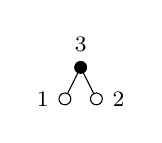
\begin{tikzpicture}[baseline=1.2mm]
    \newcommand{\sz}{2.0mm}
    \node (r1) at (-\sz, 0) [whitedot,label=left:{\footnotesize$1$}]{};
    \node (r2) at ( \sz, 0) [whitedot,label=right:{\footnotesize$2$}]{};
    \node (r3) at (   0, 2*\sz) [blackdot,label=above:{\footnotesize$3$}]{};
    \draw (r1) -- (r3) -- (r2);
  \end{tikzpicture}
  }
  + \cdots
\end{align*}

For the cavity distribution function
\begin{align*}
y(\vr;\xi)
&=
\sum_{l = 0}^\infty
\sum_{m = 0}^l
y_{l, m} \rho^l \xi^m
\\
&=
1+
\sum_{l = 1}^\infty
\sum_{m = 1}^l
y_{l, m} \rho^l \xi^m
\\
&=
  ({
  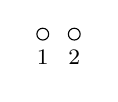
\begin{tikzpicture}[baseline=-1.0mm]
    \newcommand{\sz}{2.0mm}
    \node (r1) at (-\sz, 0) [whitedot,label=below:{\footnotesize$1$}]{};
    \node (r2) at ( \sz, 0) [whitedot,label=below:{\footnotesize$2$}]{};
  \end{tikzpicture}
  })
  +
  {
  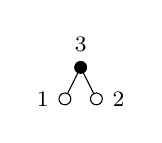
\begin{tikzpicture}[baseline=1.2mm]
    \newcommand{\sz}{2.0mm}
    \node (r1) at (-\sz, 0) [whitedot,label=left:{\footnotesize$1$}]{};
    \node (r2) at ( \sz, 0) [whitedot,label=right:{\footnotesize$2$}]{};
    \node (r3) at (   0, 2*\sz) [blackdot,label=above:{\footnotesize$3$}]{};
    \draw (r1) -- (r3) -- (r2);
  \end{tikzpicture}
  }
  + \cdots
\end{align*}


For the kernel
\begin{align*}
K(\vr;\xi)
&=
\sum_{l = 0}^\infty
\sum_{m = 1}^{l+1}
K_{l, m} \rho^l \xi^m
\\
&=
  ({
  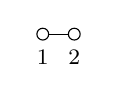
\begin{tikzpicture}[baseline=-1.0mm]
    \newcommand{\sz}{2.0mm}
    \node (r1) at (-\sz, 0) [whitedot,label=below:{\footnotesize$1$}]{};
    \node (r2) at ( \sz, 0) [whitedot,label=below:{\footnotesize$2$}]{};
    \draw (r1) -- (r2);
  \end{tikzpicture}
  })
  +
  \frac{1}{2} \,
  {
  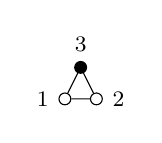
\begin{tikzpicture}[baseline=1.2mm]
    \newcommand{\sz}{2.0mm}
    \node (r1) at (-\sz, 0) [whitedot,label=left:{\footnotesize$1$}]{};
    \node (r2) at ( \sz, 0) [whitedot,label=right:{\footnotesize$2$}]{};
    \node (r3) at (   0, 2*\sz) [blackdot,label=above:{\footnotesize$3$}]{};
    \draw (r1) -- (r3) -- (r2) -- (r1);
  \end{tikzpicture}
  }
  + \cdots
\end{align*}



\subsection{Eq. (E4)}

From Eq. (E3)
\begin{align*}
  \sum_{l=0}^\infty
  \sum_{m=1}^{l+1}
  K_{l,m} \rho^l \xi^m
&=
  f
  \int_0^\xi d\xi'
  \sum_{l=0}^\infty
  \sum_{m=0}^l
  y_{l,m} \rho^l {\xi'}^m
\\
&=
  f
  \sum_{l=0}^\infty
  \sum_{m=0}^l
  y_{l,m} \rho^l \frac{ \xi^{m+1} }{m+1}
\\
&=
  \sum_{l=0}^\infty
  \sum_{m=1}^{l+1}
  \frac{ f \, y_{l,m-1} }{m} \rho^l \xi^{m}
\end{align*}

Thus
\[
  K_{l,m} = f y_{l, m-1}/m.
\]


Geometrically, for each graph in $y(\vr)$,
we join the roots by an $f$-bond,
and divide the weight by $m$,
which is number of $f$-bonds adjacent to root 1
in $y(\vr)$.



\subsection{Eq. (E5)}

From Eq. (E2)
\begin{align*}
  \sum_{l=1}^\infty
  \sum_{m=1}^{l}
  \tilde\omega_{l,m} \rho^l \xi^m
&=
  \rho
  \,
  \sum_{i=1}^\infty
  \sum_{m=1}^{i+1}
  \tilde K_{i,m} \rho^i \xi^m
 \;
  \sum_{j=0}^\infty
  \tilde h_{j} \rho^j
\\
&=
  \sum_{i=1}^\infty
  \sum_{j=0}^\infty
  \sum_{m=1}^{i+1}
  \tilde K_{i,m}
  \tilde h_j
  \, \rho^{i+j+1} \xi^m.
\end{align*}

So
\[
  \tilde \omega_{l,m}
=
  \sum_{j = 0}^{l-1}
  \tilde K_{l - j - 1, m}
  \tilde h_{j}.
\]



\subsection{Eq. (E6)}

The exponentiation satisfies $\partial_\rho y = y \partial_\rho \omega$.
\begin{align*}
\sum_{l = 1}^\infty
\sum_{m = 1}^l
l \, y_{l, m} \rho^{l-1} \xi^m
&=
\sum_{i = 0}^\infty
\sum_{n = 0}^i
y_{i, n} \rho^{i} \xi^n
\,
\sum_{j = 1}^\infty
\sum_{k = 1}^j
j \, \omega_{j, k} \rho^{j-1} \xi^k
\\
&=
\sum_{i = 0}^\infty
\sum_{n = 0}^i
\sum_{j = 1}^\infty
\sum_{k = 1}^j
j \, y_{i, n} \,
\omega_{j, k} \rho^{i+j-1} \xi^{n+k}.
\end{align*}

Thus,
\[
  l \, y_{l,m}
=
\sum_{j = 1}^{l} \sum_{k = 1}^j
j \, y_{i, n} \, \omega{j, k}.
\]
The index $k$ satisfies
\begin{align*}
   0 \le n = m - k \le i,
\end{align*}
or
\[
  m - (l - j) = m - i \le k \le m.
\]


\subsection{Eq. (E7)}

Since $1+h = g = (1+f) \,y$, we have
\[
  \sum_{l = 0}^\infty (\delta_{l,0} + h_{l}) \rho^l
=
  \sum_{l = 0}^\infty
  \left[
    (1 + f) \sum_{m = 0}^l y_{l, m} \xi^m \Big|_{\xi = 1}
  \right] \rho^l.
\]

So
\[
  \delta_{l, 0} + h_l
  = (1 + f) \sum_{m=0}^l
  y_{l, m}.
\]



\section{Appendix G: Expansion of correlation functions around a finite density}


\subsection{Recurrence relation for $[1 - (\rho + \Delta \rho) \, \tilde c]^{-1}$}

The general formula, unnumbered equation above Eq. (G1), is
%
\begin{align}
  \rho \, \tilde h_{l;\rho}
&=
\left\{
  \left[
    1 - \rho \, \tilde c
    - \sum_{i = 1}^l
        (\rho \, \tilde c_{i;\rho} + \tilde c_{i-1;\rho})
          \, \Delta \rho^i
  \right]^{-1}
\right\}_{l;\rho}
\notag \\
&\hphantom{=}- \tilde h_{l-1; \rho}.
\label{eq:oz_nzrho1}
\end{align}
%
For convenience,
we introduce
\begin{align*}
  \tilde C_i
&\equiv
  \rho \, \tilde c_{i;\rho} + \tilde c_{i-1;\rho},
\\
  \tilde H_i
&\equiv
  \rho \, \tilde h_{i;\rho} + \tilde h_{i-1;\rho},
\\
  K
&\equiv
  1 + \rho \, \tilde h
  =
  (1 - \rho \, \tilde c)^{-1},
\end{align*}
%
where
$\tilde h = \tilde h_{0;\rho}$
and
$\tilde c = \tilde c_{0;\rho}$.
%
Then, \eqref{eq:oz_nzrho1} can be rewritten as
\begin{align*}
  H_l
&=
  \left[
    \left(
      K^{-1} - \sum_{i = 1}^l C_i \, \Delta \rho^i
    \right)^{-1}
  \right]_{l;\rho}
\\
&= K
  \left[
    \left(
      1 - K \sum_{i = 1}^l C_i \, \Delta \rho^i
    \right)^{-1}
  \right]_{l;\rho}.
\end{align*}
%
or, by adding up the components,
%
\begin{align*}
  1 + K^{-1} \sum_{l = 1}^\infty H_l \, \Delta \rho^l
=
  \left(
    1 - K \sum_{i = 1}^\infty C_i \, \Delta \rho^i
  \right)^{-1}.
\end{align*}
%
Then, we have
%
\begin{align*}
  \left(
    1 + K^{-1} \sum_{l = 1}^\infty H_l \, \Delta \rho^l
  \right)
  \left(
    1 - K \sum_{i = 1}^\infty C_i \, \Delta \rho^i
  \right)
=
  1.
\end{align*}
By inspecting the coefficient of $\Delta \rho^l$, we get
\begin{align*}
  H_l
= K \sum_{i = 1}^{l - 1} H_{l - i} \, C_i + K^2 \, C_l
= K \sum_{i = 1}^{l} H_{l - i} \, C_i,
\end{align*}
where
we have defined $\tilde h_{-1;\rho} \equiv 1$,
such that $H_0 = \rho \, \tilde h_{0;\rho} + \tilde h_{-1;\rho} = K$,
or,
\begin{align}
  \rho \, \tilde h_{l;\rho}
=
  K \sum_{i = 1}^{l}
  (\rho \, \tilde h_{l-i;\rho} + \tilde h_{l-i-1;\rho})
  (\rho \, \tilde c_{i;\rho} + \tilde c_{i-1;\rho})
  - \tilde h_{l-1;\rho},
  \label{eq:hc_nzrho}
\end{align}
which is the second part of the unnumbered equation
before Eq. (G1).



\subsection{Proof of Eq. (G1)}

We now prove
\begin{equation}
  \tilde h_{l;\rho}
=
  K \, \tilde h_{l-1;\rho} \, \tilde c_{0;\rho}
+
  K \sum_{i = 1}^l (\rho \, \tilde h_{l - i;\rho} + h_{l-1-i;\rho} ) \, \tilde c_{i;\rho}.
  \label{eq:hc_nzrho_simplified}
\end{equation}
We shall do this by induction.



\subsubsection{$l=1$ case}

For $l = 1$,
we get from \eqref{eq:hc_nzrho} that
\begin{align}
\rho \, \tilde h_{1;\rho}
&=
  K \, (\rho \, \tilde h_{0;\rho} + \tilde h_{-1;\rho}) \,
  \rho \, \tilde c_{1;\rho}
+
  K \, (\rho \, \tilde h_{0;\rho} + \tilde h_{-1;\rho}) \,
  \tilde c_{0;\rho}
-
  \tilde h_{0;\rho}
\notag
\\
&=
  K^2 \,
  \rho \, \tilde c_{1;\rho}
+
  (K - 1) \, \tilde h_{0;\rho}
=
\rho (K^2 \, \tilde c_{1;\rho} + \tilde h^2 ).
\label{eq:hc_nzrho1a}
\end{align}
Note that we have used the Ornstein-Zernike relation: $\tilde h = K \tilde c$.

On the other hand, \eqref{eq:hc_nzrho_simplified}
gives
\begin{align}
  \tilde h_{1;\rho}
&=
  K \, \tilde h_{0;\rho} \, \tilde c_{0;\rho}
+
  K (\rho \, \tilde h_{0;\rho} + h_{-1;\rho} ) \, \tilde c_{1;\rho}
\\
&=
  \tilde h^2 + K^2 \, \tilde c_{1;\rho},
\label{eq:hc_nzrho1b}
\end{align}
which agrees with \eqref{eq:hc_nzrho1a}.
%
This means \eqref{eq:hc_nzrho_simplified}
holds for $l = 1$.




\subsubsection{Generally $l$}


Now suppose \eqref{eq:hc_nzrho_simplified}
holds for the $l$ case,
%
Now let us prove the $l + 1$ case.

From \eqref{eq:hc_nzrho_simplified},
we get
\begin{align*}
  \rho \, \tilde h_{l+1;\rho}
&=
  K \sum_{i = 1}^{l+1}
  (\rho \, \tilde h_{l+1-i;\rho} + \tilde h_{l-i;\rho}) \,
  \rho \, \tilde c_{i;\rho}
+
  K \sum_{i = 1}^{l+1}
  (\rho \, \tilde h_{l+1-i;\rho} + \tilde h_{l-i;\rho}) \,
  \tilde c_{i-1;\rho}
-
  h_{l;\rho}
%
%
%
\\
&=
  K \sum_{i = 1}^{l+1}
  (\rho \, \tilde h_{l+1-i;\rho} + \tilde h_{l-i;\rho}) \,
  \rho \, \tilde c_{i;\rho}
+
  K \sum_{i = 1}^{l}
  (\rho \, \tilde h_{l-i;\rho} + \tilde h_{l-1-i;\rho}) \,
  \tilde c_{i;\rho}
\\
&\hphantom{=\quad}
+ K \,
  (\rho \, \tilde h_{l;\rho} + \tilde h_{l-1;\rho}) \,
  \tilde c_{0;\rho}
-
  h_{l;\rho}
%
%
%
\\
&=
  K \sum_{i = 1}^{l+1}
  (\rho \, \tilde h_{l+1-i;\rho} + \tilde h_{l-i;\rho}) \,
  \rho \, \tilde c_{i;\rho}
+ K \,
  \rho \, \tilde h_{l;\rho} \,
  \tilde c_{0;\rho}
\\
&\hphantom{=\quad}
+
\left[
  K \sum_{i = 1}^{l}
  (\rho \, \tilde h_{l-i;\rho} + \tilde h_{l-1-i;\rho}) \,
  \tilde c_{i;\rho}
+ K \,
  \tilde h_{l-1;\rho} \,
  \tilde c_{0;\rho}
-
  h_{l;\rho}
\right].
%
%
%
\end{align*}
The terms in the square brackets vanish because of the induction hypothesis,
\eqref{eq:hc_nzrho_simplified};
the remaining terms give
\eqref{eq:hc_nzrho_simplified}
for the $l + 1$ case.
This completes the proof of
\eqref{eq:hc_nzrho_simplified}.




\subsection{The $l = 1$ case}

From \eqref{eq:hc_nzrho1b},
we get
\begin{align*}
\partial_\rho \tilde t
&=
\partial_\rho \tilde h
-
\partial_\rho \tilde c
\\
&=
\tilde h^2
+
\rho \, \tilde h \,
(2 + \rho \, \tilde h) \,
\partial_\rho \tilde c.
\end{align*}



\section{Appendix H.}



\subsection{H.5 RH theorem}



The first paragraph states the generalized RH theorem.
%
The generalized RH theorem applies to any fluid
not just hard spheres.
%
In other words, we do not require the $f$-bond
to be either $-1$ or $0$.
%
The only property used here is $1 = e - f$,
which is always valid.

The theorem can be generalized to uniform sums of
the Mayer diagrams,
or conversely to compute the equivalent Mayer sum
of a uniform RH sum.
%
These generalizations are not discussed here
for they find no application for the present purpose.



\section{Supplemental material}

\subsection{Eq. (8)}

We start from the two function case.
%
\begin{align}
& \hphantom{=\int} (a_1 * a_2)(\vr)
\notag \\
&=
  \int_{\vr'}
    a_1(\vr') \,
    a_2(\vr - \vr') \, d\vr'
\notag \\
&=
  \int_{\vr'}
    \left(
      \int_\vk \tilde{a}_1(\vk) \, \exp(i\vk\cdot\vr') \, \dvk
    \right)
%\notag \\
%&\hphantom{=}
%\quad \times
    a_2(\vr - \vr') \, d\vr'
\notag \\
&=
  \int_\vk \dvk \,
  \tilde{a}_1(\vk) \,
  \exp(i\vk\cdot\vr)
\notag \\
&\hphantom{=}\times
  \int_{\vr'} d\vr' \,
    a_2(\vr - \vr') \, \exp[-i\vk\cdot(\vr - \vr')]
\notag \\
&=
  \int_\vk \dvk \,
  \tilde{a}_1(\vk) \,
  \tilde{a}_2(\vk) \,
  \exp(i\vk\cdot\vr).
  \label{eq:convol}
\end{align}
Thus, the Fourier transform of $a_1 * a_2$ is
$\tilde{a}_1(\vk) \, \tilde{a}_2(\vk)$:
\[
  \FT(a_1 * a_2)(\vk) = \tilde{a_1}(\vk) \, \tilde{a}_2(\vk).
\]

It follows that
\begin{align*}
  \FT(a_1 * a_2 * a_3)(\vk)
&= \FT(a_1 * a_2)(\vk) \, \tilde{a}_3(\vk)
  \\
&= \tilde{a}_1(\vk) \, \tilde{a}_2(\vk) \, \tilde{a}_3(\vk).
\end{align*}
and by induction
\begin{align*}
  \FT(a_1 * \cdots * a_l)(\vk)
&= \tilde{a}_1(\vk) \, \cdots \, \tilde{a}_l(\vk).
\end{align*}

This means
\begin{align*}
  (a_1 * \cdots * a_l)(\vr)
= \int \dvk \, \tilde{a}_1(\vk) \, \cdots \, \tilde{a}_l(\vk)
  \, \exp(i\vk\cdot\vr).
\end{align*}
%
Now setting $\vr = 0$ yields the first equality.
\begin{align*}
  (a_1 * \cdots * a_l)(\vct 0)
= \int \dvk \, \tilde{a}_1(\vk) \, \cdots \, \tilde{a}_l(\vk).
\end{align*}

Setting $\vr = 0$ in the first expression of \eqref{eq:convol}, yields
\[
  \int a_1(\vr') \, a_2(-\vr') \, d\vr'
= \int \dvk \tilde{a}_1(\vk) \, \tilde{a}_2(\vk).
\]
For an even $a_2$,
the left hand side can be written as
\[
  \int a_1(\vr) \, a_2(\vr) \, d\vr.
\]



\subsection{Derivatives w.r.t. $\zeta$ in the PY equation}



For $\partial_\zeta c$,
we have $c + t = (1 + f) \, y$,
with $y = 1 + t$,
and
\begin{align*}
\partial_\zeta c
+ \partial_\zeta t
&= \partial_\zeta [(1+f)y]
=
(1 + f) \partial_\zeta t
+ (1 + t) \, \partial_\zeta f.
\end{align*}

So
\begin{align}
\partial_\zeta c
=
f \, \partial_\zeta t
+ (1+t) \partial_\zeta f.
\label{eq:dcdzeta}
\end{align}

Using \eqref{eq:dcdzeta},
\begin{align*}
  t\, \partial_\zeta c - c \, \partial_\zeta t
&=
  t \, f \, \partial_\zeta t
+ t \, (1 + t) \, \partial_\zeta f
- f \, (1 + t) \, \partial_\zeta t
\\
&=
- f \, \partial_\zeta t
+ t \, (1 + t) \, \partial_\zeta f.
\end{align*}


\subsection{Simplified PY pressure, hard-sphere simplification}

The relation $S_D/(2D) = B_2$ comes from \eqref{eq:B2v}.


\subsection{$\partial_\zeta c$ in the HNC equation}

For $\partial_\zeta c$, we have
$c + t = (1 + f) \, y$
with
$y = \exp t$,
and
\begin{align*}
  \partial_\zeta c + \partial_\zeta t
&= (1 + f) \, \partial_\zeta y
+ y \, \partial_\zeta f
\\
&= (1 + f) \, y \, \partial_\zeta t
+ y \, \partial_\zeta f
\\
&= (1 + c + t) \, \partial_\zeta t
+ y \, \partial_\zeta f
\end{align*}

So
\begin{align*}
  \partial_\zeta c
&= (c + t) \, \partial_\zeta t
+ y \, \partial_\zeta f.
\end{align*}


\bibliography{liquid}
\end{document}

